%%%%%%%%%%%%%%%%%%%%%%%%%%%%%%%%%%%%%%%%%%%%%%%%%%%%%%%%%%%%%%%%%%%%%%%%%%%%%%%%
%2345678901234567890123456789012345678901234567890123456789012345678901234567890
%        1         2         3         4         5         6         7         8

\documentclass[letterpaper, 10 pt, conference]{ieeeconf}  % Comment this line out if you need a4paper


%\documentclass[a4paper, 10pt, conference]{ieeeconf}      % Use this line for a4 paper

\IEEEoverridecommandlockouts                              % This command is only needed if 
                                                          % you want to use the \thanks command

\overrideIEEEmargins                                      % Needed to meet printer requirements.

%In case you encounter the following error:
%Error 1010 The PDF file may be corrupt (unable to open PDF file) OR
%Error 1000 An error occurred while parsing a contents stream. Unable to analyze the PDF file.
%This is a known problem with pdfLaTeX conversion filter. The file cannot be opened with acrobat reader
%Please use one of the alternatives below to circumvent this error by uncommenting one or the other
%\pdfobjcompresslevel=0
%\pdfminorversion=4

% See the \addtolength command later in the file to balance the column lengths
% on the last page of the document

% The following packages can be found on http:\\www.ctan.org
%\usepackage{graphics} % for pdf, bitmapped graphics files
%\usepackage{epsfig} % for postscript graphics files
%\addbibresource{references.bib}
\usepackage{multicol}
%\usepackage[bookmarks=true]{hyperref}
\usepackage[utf8]{inputenc} % allow utf-8 input
\usepackage[T1]{fontenc}    % use 8-bit T1 fonts
\usepackage{hyperref}       % hyperlinks
\usepackage{url}            % simple URL typesetting
\usepackage{booktabs}       % professional-quality tables
\usepackage{amsfonts}       % blackboard math symbols
\usepackage{nicefrac}       % compact symbols for 1/2, etc.
\usepackage{microtype}      % microtypography
\usepackage{epigraph}
\usepackage{graphicx}
\usepackage{amsmath}
\usepackage{array}
\usepackage{hyperref}
\usepackage[binary-units=true]{siunitx}
\usepackage{subcaption}
\usepackage{bm}
\usepackage{mathtools}
\usepackage{cuted}
\usepackage{etoolbox}
\usepackage{balance}
\usepackage{multirow}

\usepackage{wrapfig}

\newcommand\mypara[1]{\vspace{3pt}\noindent\textbf{#1.}}
\newcommand{\propose}[1]{\textcolor{blue}{#1}}
\newcommand{\todo}[1]{\textcolor{red}{TODO: #1}}
% tex2plot

\usepackage{pgfplots}
\pgfplotsset{compat=newest}
%% the following commands are needed for some matlab2tikz features
\usetikzlibrary{plotmarks}
\usetikzlibrary{babel}
\usetikzlibrary{arrows.meta}
\usepgfplotslibrary{patchplots}
\usepackage{grffile}
\usepackage{amsmath}
\usepackage{interval}

\usepgfplotslibrary{groupplots}
\usepgfplotslibrary{dateplot}
%\usepackage{mathptmx} % assumes new font selection scheme installed
%\usepackage{times} % assumes new font selection scheme installed
%\usepackage{amsmath} % assumes amsmath package installed
%\usepackage{amssymb}  % assumes amsmath package installed

% Learning vision based locomotion by walking blind
% Learning too see by walking blind
% Learning Vision for Walking
% Self supervised visual learning for locomotion
% Self supervised learning of vision for walking
% learning vision for walking from proprioception
% Learning Vision from proprioception for walking


\title{\LARGE \bf
% Rapidly Adapting Quadcopter Controllers:\\ One Policy to Fly Them All
% Scaling Up Adaptation for Quadcopters
% Universal Quadcopter Controllers:\\A Learning Approach for Zero-shot Adaptive Quadcopter Control
% A Zero-Shot Adaptive Quadcopter Controller
Learning a Single Near-hover Position Controller\\for Vastly Different Quadcopters
% An adaptive controller for quadcopters capable of compensating for extreme parameter variations
}

\author{Dingqi Zhang$^1$, Antonio Loquercio$^2$, Xiangyu Wu$^1$, Ashish Kumar$^2$, Jitendra Malik$^2$, and Mark W. Mueller$^1$% <-this % stops a space
%\thanks{*This work was not supported by any organization}% <-this % stops a space
\thanks{The authors are with the $^1$High Performance Robotics Lab, Dept. of Mechanical Engineering, and the $^2$Dept. of Electrical Engineering and Computer Science, University of California Berkeley, \{dingqi, loquercio, wuxiangyu, ashish\_kumar, malik, mwm\}@berkeley.edu} 
% \thanks{$^{2}$Bernard D. Researcheris with the Department of Electrical Engineering, Wright State University,
%         Dayton, OH 45435, USA
%         {\tt\small b.d.researcher@ieee.org}}%
}


\begin{document}


\maketitle
\maketitle
\thispagestyle{empty}
\pagestyle{empty}

% \todo{formatting to fit 6+n}

% \todo{•	How do you initialize the history to estimate z in the real world. Specifically, what are the initial history to generate z, or how do you generate z for the first iteration?}

% \todo{I think similar to [1] you could do a PCA analysis on the embedding space to see how the mass or other parameters affect the embedding. }

% \todo{ Why did you use a 3-layer 1-D cnn for the adaption module, rather then a more sequential based model (which seems to fit well for the time-based nature of the data), for example a LSTM or Transformer.  }

% \todo{Minor Correction (Typos, etc.) Sec II, Paragraph 2: Define the intrinsics vector before using the term in passing.}

% \todo{The main criticisms involve the need of narrowing down the main contributions as well as the comparison to earlier work. In the event that these two criticisms are tackled, the paper might be suitable for publication.}

%%%%%%%%%%%%%%%%%%%%%%%%%%%%%%%%%%%%%%%%%%%%%%%%%%%%%%%%%%%%%%%%%%%%%%%%%%%%%%%%
\begin{abstract}
This paper proposes an adaptive near-hover position controller for quadcopters, which can be deployed to quadcopters of very different mass, size and motor constants, and also shows rapid adaptation to unknown disturbances during runtime. The core algorithmic idea is to learn a single policy that can adapt online at test time not only to the disturbances applied to the drone, but also to the robot dynamics and hardware in the same framework.
We achieve this by training a neural network to estimate a latent representation of the robot and environment parameters, which is used to condition the behaviour of the controller, also represented as a neural network. We train both networks exclusively in simulation with the goal of flying the quadcopters to goal positions and avoiding crashes to the ground. We directly deploy the same controller trained in the simulation without any modifications on two quadcopters in the real world with differences in mass, size, motors, and propellers with mass differing by 4.5 times. In addition, we show rapid adaptation to sudden and large disturbances up to one-third of the mass of the quadcopters. We perform an extensive evaluation in both simulation and the physical world, where we outperform a state-of-the-art learning-based adaptive controller and a traditional PID controller specifically tuned to each platform individually. Video results can be found at~\url{https://youtu.be/U-c-LbTfvoA}.
% Video results can be found \todo{at~\url{https://youtu.be/3yQrDML5aWs}}. %We will release our code and trained model upon acceptance.

\end{abstract}

% \makeatletter
% \g@addto@macro\@maketitle{
% \centering




% \vspace{-0.1in}
% \bigskip}
% \makeatother
% \textcolor{red}{We never use the second person ("you") in a paper. A paper isn't addressed at anyone, it is simply a report.}


%%%%%%%%%%%%%%%%%%%%%%%%%%%%%%%%%%%%%%%%%%%%%%%%%%%%%%%%%%%%%%%%%%%%%%%%%%%%%%%%
%===============================================================================

\section{Introduction}

\begin{figure}
    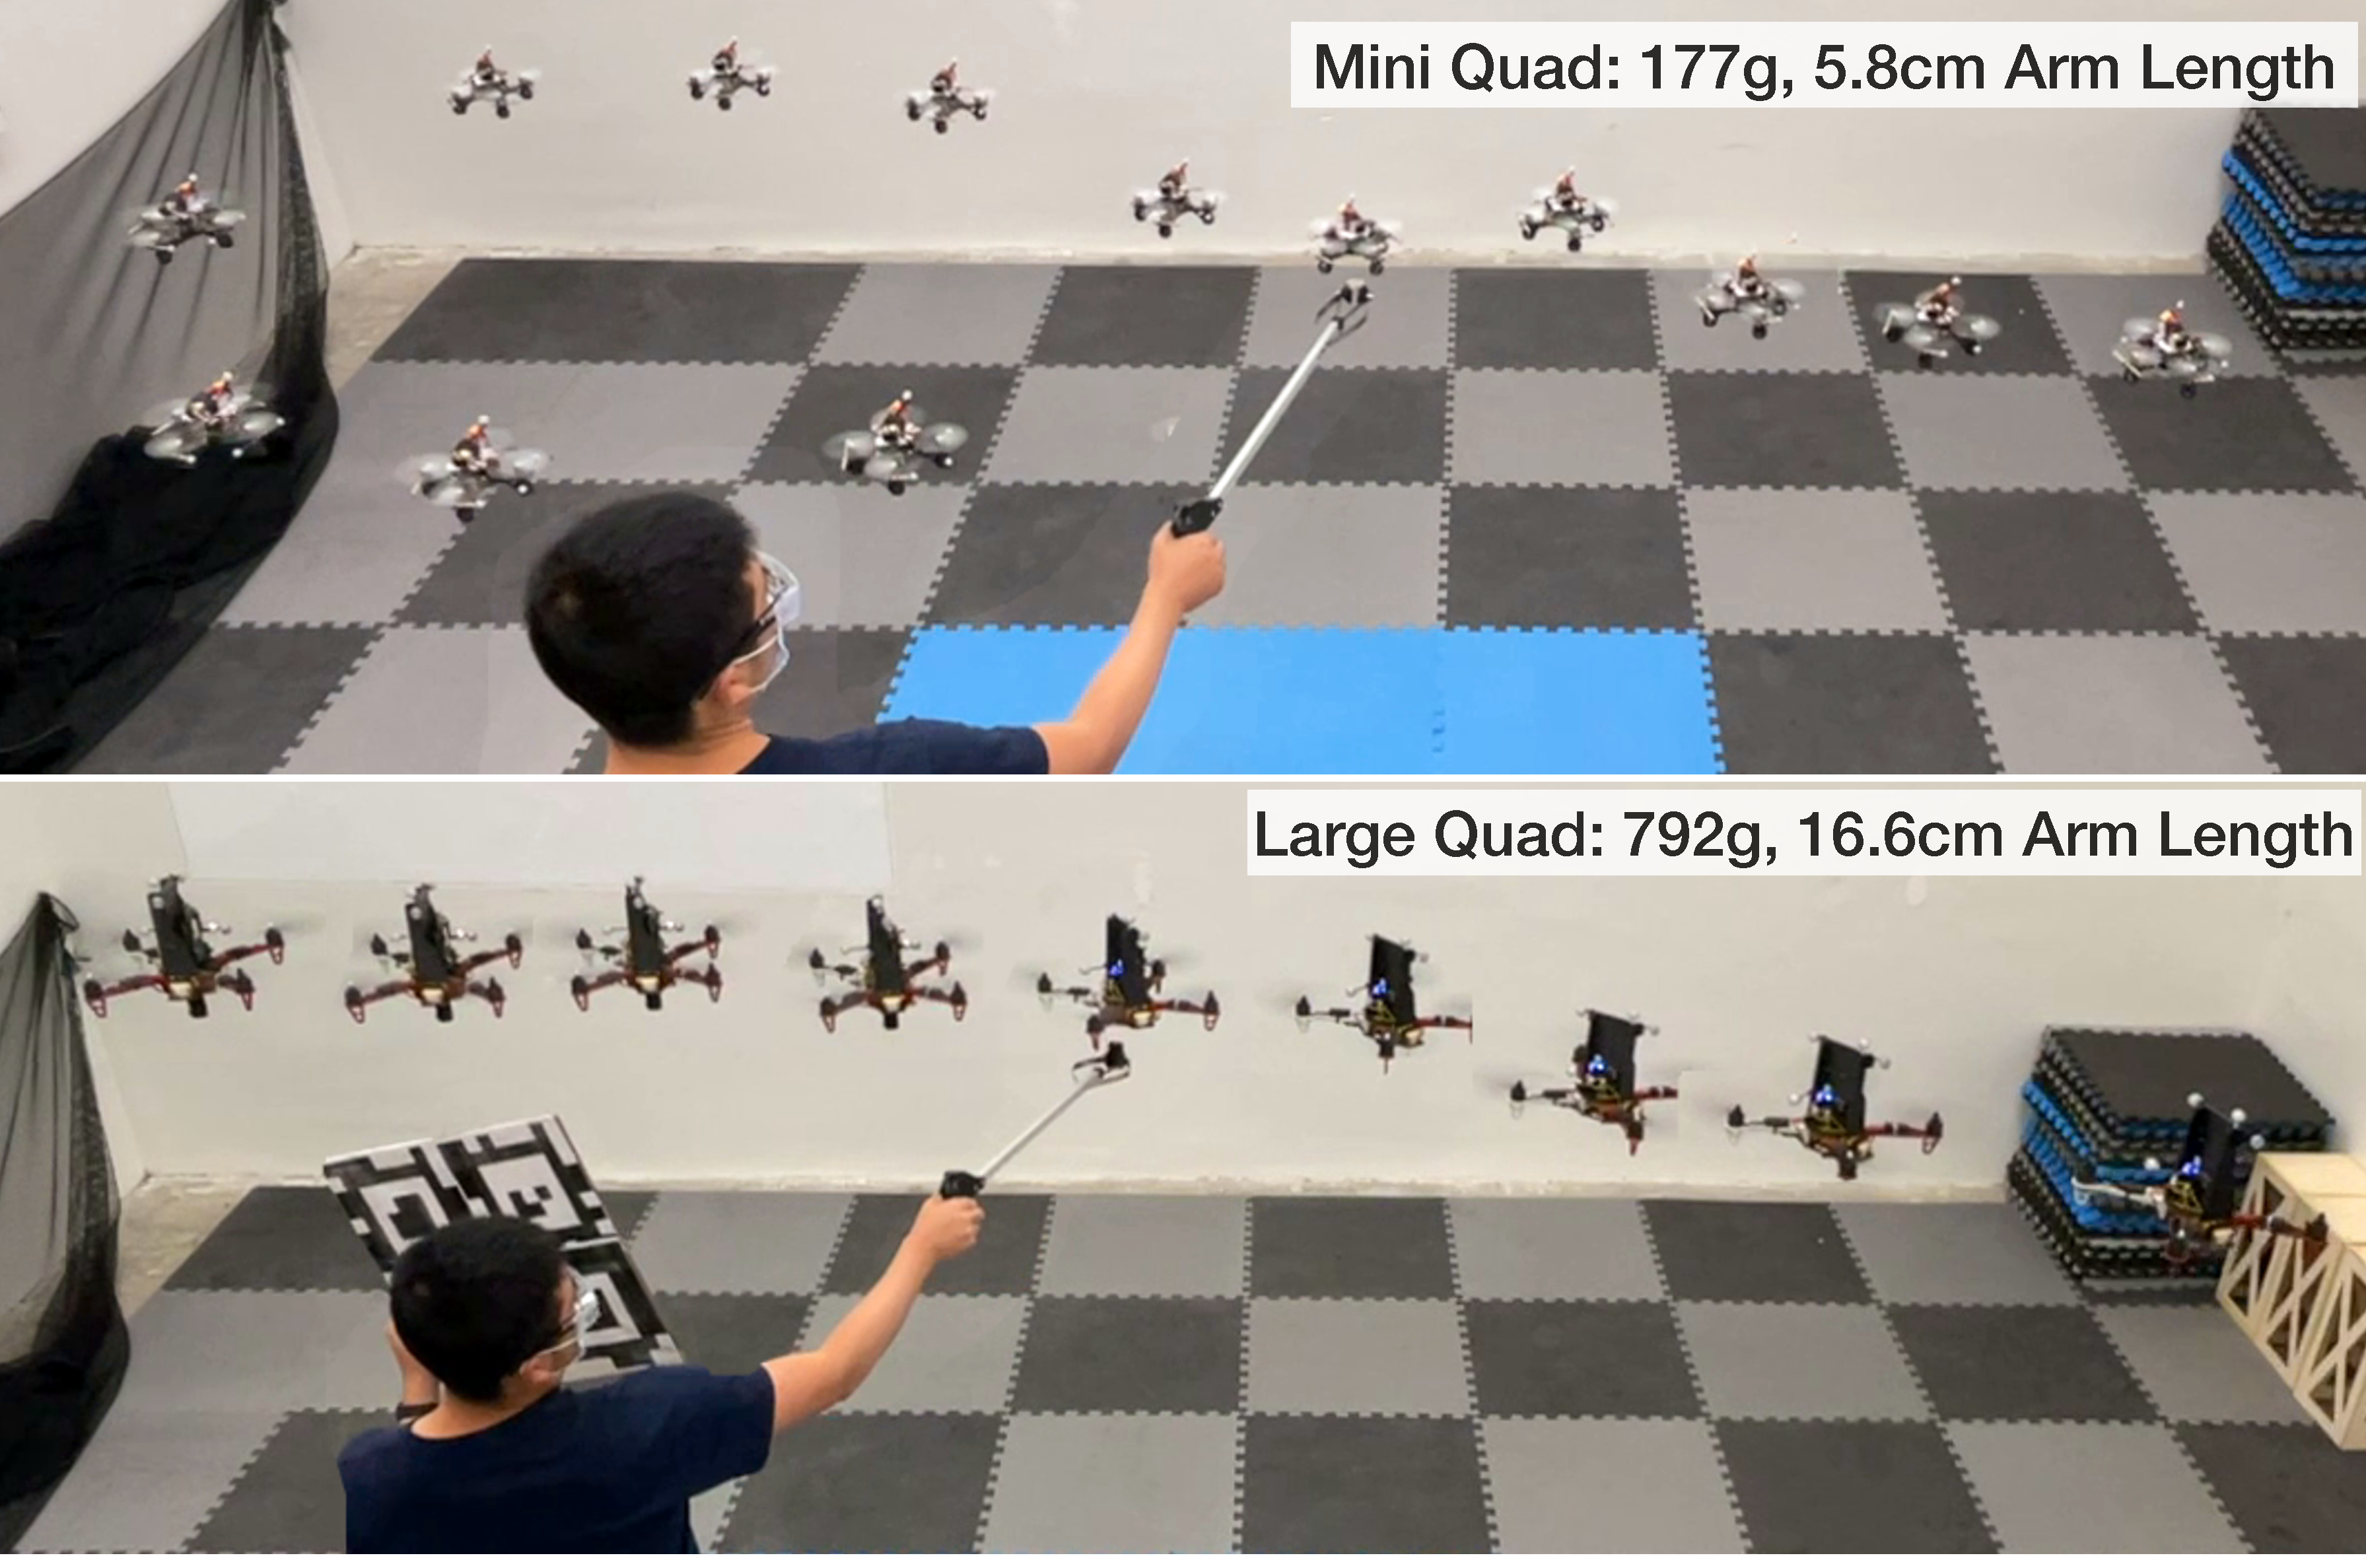
\includegraphics[width=\columnwidth]{img/figure1.pdf}
\captionof{figure}{\small Demonstration of our adaptive controller on two quadrotors with widely varying mass, arm length, and motor constants for the task of tracking a straight and circular trajectory. In the middle of the trajectory, we add a payload unknown to the drone of approximately 30\% of the robot's mass. Our end-to-end controller is able to quickly estimate and react to the disturbance. In both the demonstrations described above and all the simulation and real-world experiments presented here, we use a single control policy across different drones and tasks, which is deployed without any modifications or tuning.}
\label{fig:teaser}
\vspace{-3ex}
\end{figure}

% \todo{change the notation of low level controller}

% \propose{\begin{itemize}
%     \item in robotics field, we have good solutions in specific tasks. 
%     \item gives rise to an idea for general purpose solution 
%     \item we think this problem in quadcopter controller settings
%     \item quadcopters are good in easy access and wide range of application  
%     \item a good controller need knowledge of the model and careful tuning 
%     \item traditional (PID), RL, all control them well
%     \item However, they are platform-specific. often fails when transferring to new models. need start from scrach training for learning controller, or specific tuning for traditional 
%     \item In addition, disturbance rejection are usually applied on the specific model and on specific disturbance. (need reference)
%     \item rejection to different disturbance, requires extensive data collections and simulated models  
%     \item a universal controller applied to different quadcopters to save the labor intensive work. And on general disturbances rejection at the same time.
%     \item Our controller is able to adapt based not only on morphology, but also down to hardware characteristic (one level higher).
% \end{itemize}}
% 
% \propose{\begin{itemize}
%     \item Adaptive control is cool and works (ref)
%     \item However, under the hood, those methods assume access to the underlying model of the platform and hardware.
%     \item This assumption is justified in a industrial setting (where all drones are the same).
%     \item However, what happens if we lift such assumption?
%     \item Why is this question important? Example: hobby or research drones (cite the several flight stacks).
%     \item Doing so requires a "universal" controller, that can adapt not only to disturbances, but also to the morphology and hardware of the robot.
%     \item In this paper, we use a learning-based adaptive controller to solve this problem.
%     \item The controller is robust to unseen disturbances at train time.
%     \item This approach works better than existing methods.
%     \item We extensively test it in both sim and real world.
% \end{itemize}
%
%Adaptive control for aerial vehicles has been a top priority for research for decades. 
% %
% It has achieved great access in extensive scales of applications from an indoor quadcopter~\cite{hanover2021performance} to a civil transport aircraft~\cite{doi:10.2514/6.2009-5738}.
% %
% However, with its approaches greatly evolving, it assumes access to the underlying model of the platform and hardware.
% %
% Adaptive control is greatly concerned with estimating and conteracting disparities between observation and a \emph{reference} model. 
% %
% This assumption leads one to wonder: what happens if we can lift such assumption? 
% %
% If so, the controller can completely bypass the notion of a reference model, which enables adaptation not only to disturbances and model uncertainties, but also to the morphology and hardware of the robot. 
% %
% This much wider range of adaptation can greatly save the labor-intensive process of designing controllers for quadcopters.
% %
% % Recent years have witnessed the growing interest in quadcopters due to its versatility in applications.
% % %
% % Such growing interest has lead to the emergence of commercially available and customizable quadcopters for hobbyists and researchers. 
% %
% Designing optimal controllers for quadcopters is challenging, as it requires accurate knowledge of the dynamics of quadcopters and careful controller design for desired skills. (basically copied from locomotion paper)
% %
% Poorly designed controllers can lead to suboptimal performances for quadcopters. In some cases, they may even become potentially danguerous for quadcopters such highly dynamic systems, since failure to control quickly leads to a crash. 
% %
% Flight stacks like PX4~\cite{PX4} and Beta-Flight~\cite{BetaFlight} have enabled the design process easier, but they still requires significant in-flight tuning for each quadcopter type and are generally tailored to human pilots. 
% %
% %
% }

% \propose{
% \begin{enumerate}
%     \item Optimal control of quadcopter requires a delicate design of controller. 
%     \item This controller requires accurate model estimtion.
%     \item Laborious procedure description 
%     \item Laborious procedure will be eased if a single controller exists. 
%     \item Not existed, because it's hard with unstable dynamics.
%     \item Model uncertainty and disturbance rejection requires more layer of complexity
% \end{enumerate}
% }

% \todo{The joy of the design and assembly of a new quadcopter is generally followed by great despair.
% %
% Once the hardware is in place, getting the quadcopter into the air may apparently look like a simple task.
% %
% Well-established systems provide a simple way for generating trajectories and high-level controllers for tracking them (e.g., \cite{mueller2019trajectory,mellinger2012trajectory,kaufmann2020RSS}).
% %
% Such high-level controllers generally abstract action in terms of thrust and angular rates.
% %
% The interface between these actions and motor commands, physically executable by the hardware, is an \emph{appropriate} low-level controller. % that, e.g., meet certain specification on closed-loop time constants.
% %
% And here is where the headaches start.}

A classic controller for quadcopters requires explicit estimates of the vehicle's model, including inertia properties (MMOI and mass), motor constants, and other parameters.
%
Errors in estimating such parameters directly translate to errors in the execution of the controller commands.
%
In addition, once the parameters are estimated, the controller requires specific tuning in-flight to achieve the desired behaviour.
%
% If the estimation and tuning is done right, the final performance will be very good.
%
% But what looked like a simple task required significant engineering effort.
%
A small modification to the vehicle, e.g., replacing the motors with ones that have different properties or a different shape, would require repeating the above steps in estimation and tuning.
%
Such significant engineering efforts could be eased with a single controller without specialized tuning. However, this problem raises several challenges since quadcopters are very unstable systems. 
%
Large variations in quadcopter design have prompted the design of specialized controllers for different quadcopters, as opposed to one single controller. 
%
Rejection to disturbances or model uncertainties requires non-trivial design changes to the specialized controllers, which add more layers of complexity to the design work.
%
% Such engineering effort is compounded when the vehicle has variable properties, e.g., can carry different payloads or has a changing shape~\cite{falanga2018foldable,derrouaoui2022adaptive}.
% %
% Moreover, additional engineering effort and tuning is required if the controller needs to be robust against model uncertainties or external disturbances, e.g. aerodynamics effects or wind~\cite{shi2019neural, neuralfly, torrente2021data}.

% \todo{Introduction
% This section could be better organized to motivate why a
% universal controller is important, and why existing
% approaches do not serve as universal controllers. More
% specifically:
% Organization:
% Authors should provide motivation (e.g. autopilot without
% tuning) in the first paragraph before beginning a
% discussion on why the universal control problem is
% technically challenging.
% Authors should briefly state what their universal
% controller actually accomplishes (e.g. low-level control of
% thrust and angular velocity), which is not clear in the
% introduction.
% Discussion related to the technical challenge of the
% problem is scattered through the introduction and can be
% consolidated. 
% The reasoning behind why past approaches are not
% universal drone controllers should be better justified.}

% In this paper, we show the first universal controller for quadcopters. 
% %
% Quadcopters are inherently unstable and require high-frequency control of up to 500Hz. 
% %
% Failure to adapt to perturbations within fractions of a second can potentially lead to a crash.
% %
% Consequently, a universal controller should not only be able to handle diverse perturbations, it should do so very fast. 
%
% \todo{The introduction indicates that the controller is able to adapt to new situations within 0.8 sec (which corresponds to the window of 400 steps). But in Section V.C, empirical results indicate that the adaptation period is close to 2 secs.}
% 
In this work, we show the first controller aiming to control a variety of quadcopters with differences in mass, armlength, motor constant, etc. of up to 4 times within one second, without any modification or fine-tuning for the specific quadcopters. Our controller is a near-hover position controller capable of flying vastly different quadcopters to target positions.
%
In addition, our controller can rapidly adapt to unknown disturbances in the mass and inertia changes of the quadcopters.
%
Our work builds on three main insights.
%
The first is that the dynamics parameters are observable from the history of states and actions.
%
This has long been known in the community: several works have shown how to estimate parameters online with filters~\cite{svacha2020imu,wuest2019online} or with neural networks~\cite{forgione2021continuous}.
%
Yet, prior work overlooked the possibility of using these estimates to condition the controller's behaviour.
%
The second insight is that, at test time, we do not need an estimate of the parameters in some "ground truth" sense.
%
What matters is that the estimate leads to the "right" action, which our end-to-end training procedure optimizes.
%
This simplifies the estimation problem and avoids identifiability issues, e.g., identical effects on unobservable or unmatched uncertainties~\cite{hovakimyan2010l1}.
%
% The third and final insight is that a system trained to adapt to a large variety of morphological and dynamical parameters is automatically robust to disturbances which are very difficult to model and to train on, \emph{e.g}, aerodynamics effects or swinging payloads.
%
% \todo{When the authors enumerate the three insights leveraged by their algorithm, the third comment about the algorithm being robust to disturbances within the convex hull of the training should be substantiated. }
%
The third and final insight is that a system can adapt to previously unseen disturbances as long as their effect on the platform dynamics is in the convex hull of the training disturbances (e.g., a motor losing efficiency has a similar effect to adding a payload below the motor).
%Therefore, future work should not spend effort on simulating all possible disturbances but on finding the minimal set of parameter changes to trigger a reaction.}
% we can train both the controller and the latent parameter identification module in simulation, where both the ground truth values and the state-action history are available. \antonio{The last insight is a bit less "insightful" than the others, maybe remove?}

To operationalize this, we follow the approach initially proposed for legged robots~\cite{kumar2021rma}. However, while this work performs online adaptation to terrains, we use their approach to adapt to a diverse set of quadcopter bodies and perturbations. Specifically, we estimate a latent representation of the quadcopter's body from a history of sensor observations and actions, which conditions the behaviour of the controller.
%
%Such representation conditions the behaviour of the low-level controller.
The space of quadcopter properties in which we train is extremely diverse (Table~\ref{tab:randomization}).
%
%\antonio{The flow here is okaish, but don't know how to improve it}.
%
This diversity enables adaptation to sudden changes in environment conditions, e.g., a payload, for which it was not explicitly trained.
%
Our approach frees drone designers from the estimation and tuning process required any time something changes, or the risk that parameter changes unwittingly cause the control behaviour to significantly change, potentially endangering the system.
%
Furthermore, it naturally lends itself for use in off-the-shelf autopilot systems, allowing users who might otherwise lack the modelling abilities to control a custom vehicle, simply by plugging in the autopilot and not requiring any parameter tuning.

% \begin{itemize}
%     \item You get a new quadcopter.
%     \item You want it to perform a simple trajectory tracking task, and have access to any one of a number of well-established trajectory generation and high-level control (e.g., \cite{mueller2019trajectory}). These high-level controllers often treat as control input the vehicle angular velocity, which is assumed to be tracked by an appropriate low-level control that, e.g., meet certain specification on closed-loop time constants.  
%     \item Such low-level control requires estimates of vehicle inertia properties (MMOI and mass), motor constants, and other parameters; errors in estimating such parameters directly translate to errors in the low-level tracking performance. 
%     \item Once these are estimated, the controller is typically tuned in-flight to achieve the desired behaviour.
%     \item If you do all steps right, you get a good controller. But what was supposed to be a simple task required significant energy and engineering effort, and modifying the vehicle (e.g., by replacing the motors with ones that have different properties, and different mass) would require repeating the above steps.
%     Moreover, if the vehicle has variable properties (e.g., can carry different payloads) the effort is compounded.
% \end{itemize}


% \begin{itemize}
%     %\item In this paper, we propose a way to escape this important yet tedious step
%     %\item we propose a learning-based controller that can autonomously adapt to a new vehicle or to changing parameters
%     %\item To do so, our approach estimates a latent representation of the quadcopter's body from an history of sensor observations and actions.
%     %\item Such representation conditions the behaviour of the low-level controller.
%     %\item Not only can our approach quickly adapt to a new body, but also react to sudden changes in environmental conditions, e.g. wind, a payload, etc, for which it was not explicitly trained for.
%     % \item Such an approach potentially allows for a much larger exploration in the drone design, since designers do not have to repeat the estimation and tuning process any time something changes.
%     % Furthermore, the approach naturally lends itself for use in off-the-shelf autopilot systems, allowing users who might otherwise lack the modelling abilities to implement a low-level controller on a custom vehicle, simply by plugging in the autopilot and not requiring any parameter tuning. 
% \end{itemize}


%\begin{itemize}
    %\item The first insight behind our work is that the body parameters are observable from the state action history.
    %\item This has long been known in community, with several work showing how to estimate parameters online.
    %\item While this can be done with filters, or with NN. The first is provable under assumption, the second general works across a larger variety of dynamics.
    %\item NN are also especially good at estimating parameters and at working over across dynamics.
    %\item Yet, prior work overlooked the possibility of estimating those parameters \textbf{at test time} and use them to condition the low-level controller.
    %\item The second insight is that we do not need to explicitly estimate the parameters.
    %\item What we need is a low-dimensional projection of them which is relevant for control. 
    %\item If a change in payload or inertia exhibit the same form of disturbance to the quadcopter, they need to be projected to the same point in the manifold.
    %\item This largely simplifies the estimation effort at test time.
    %\item The third and final insight of our work is that we can try both the controller and the latent body identification module in simulation, where both the ground truth parameters and the state-action history are available.
%\end{itemize}

\begin{figure}
\centering
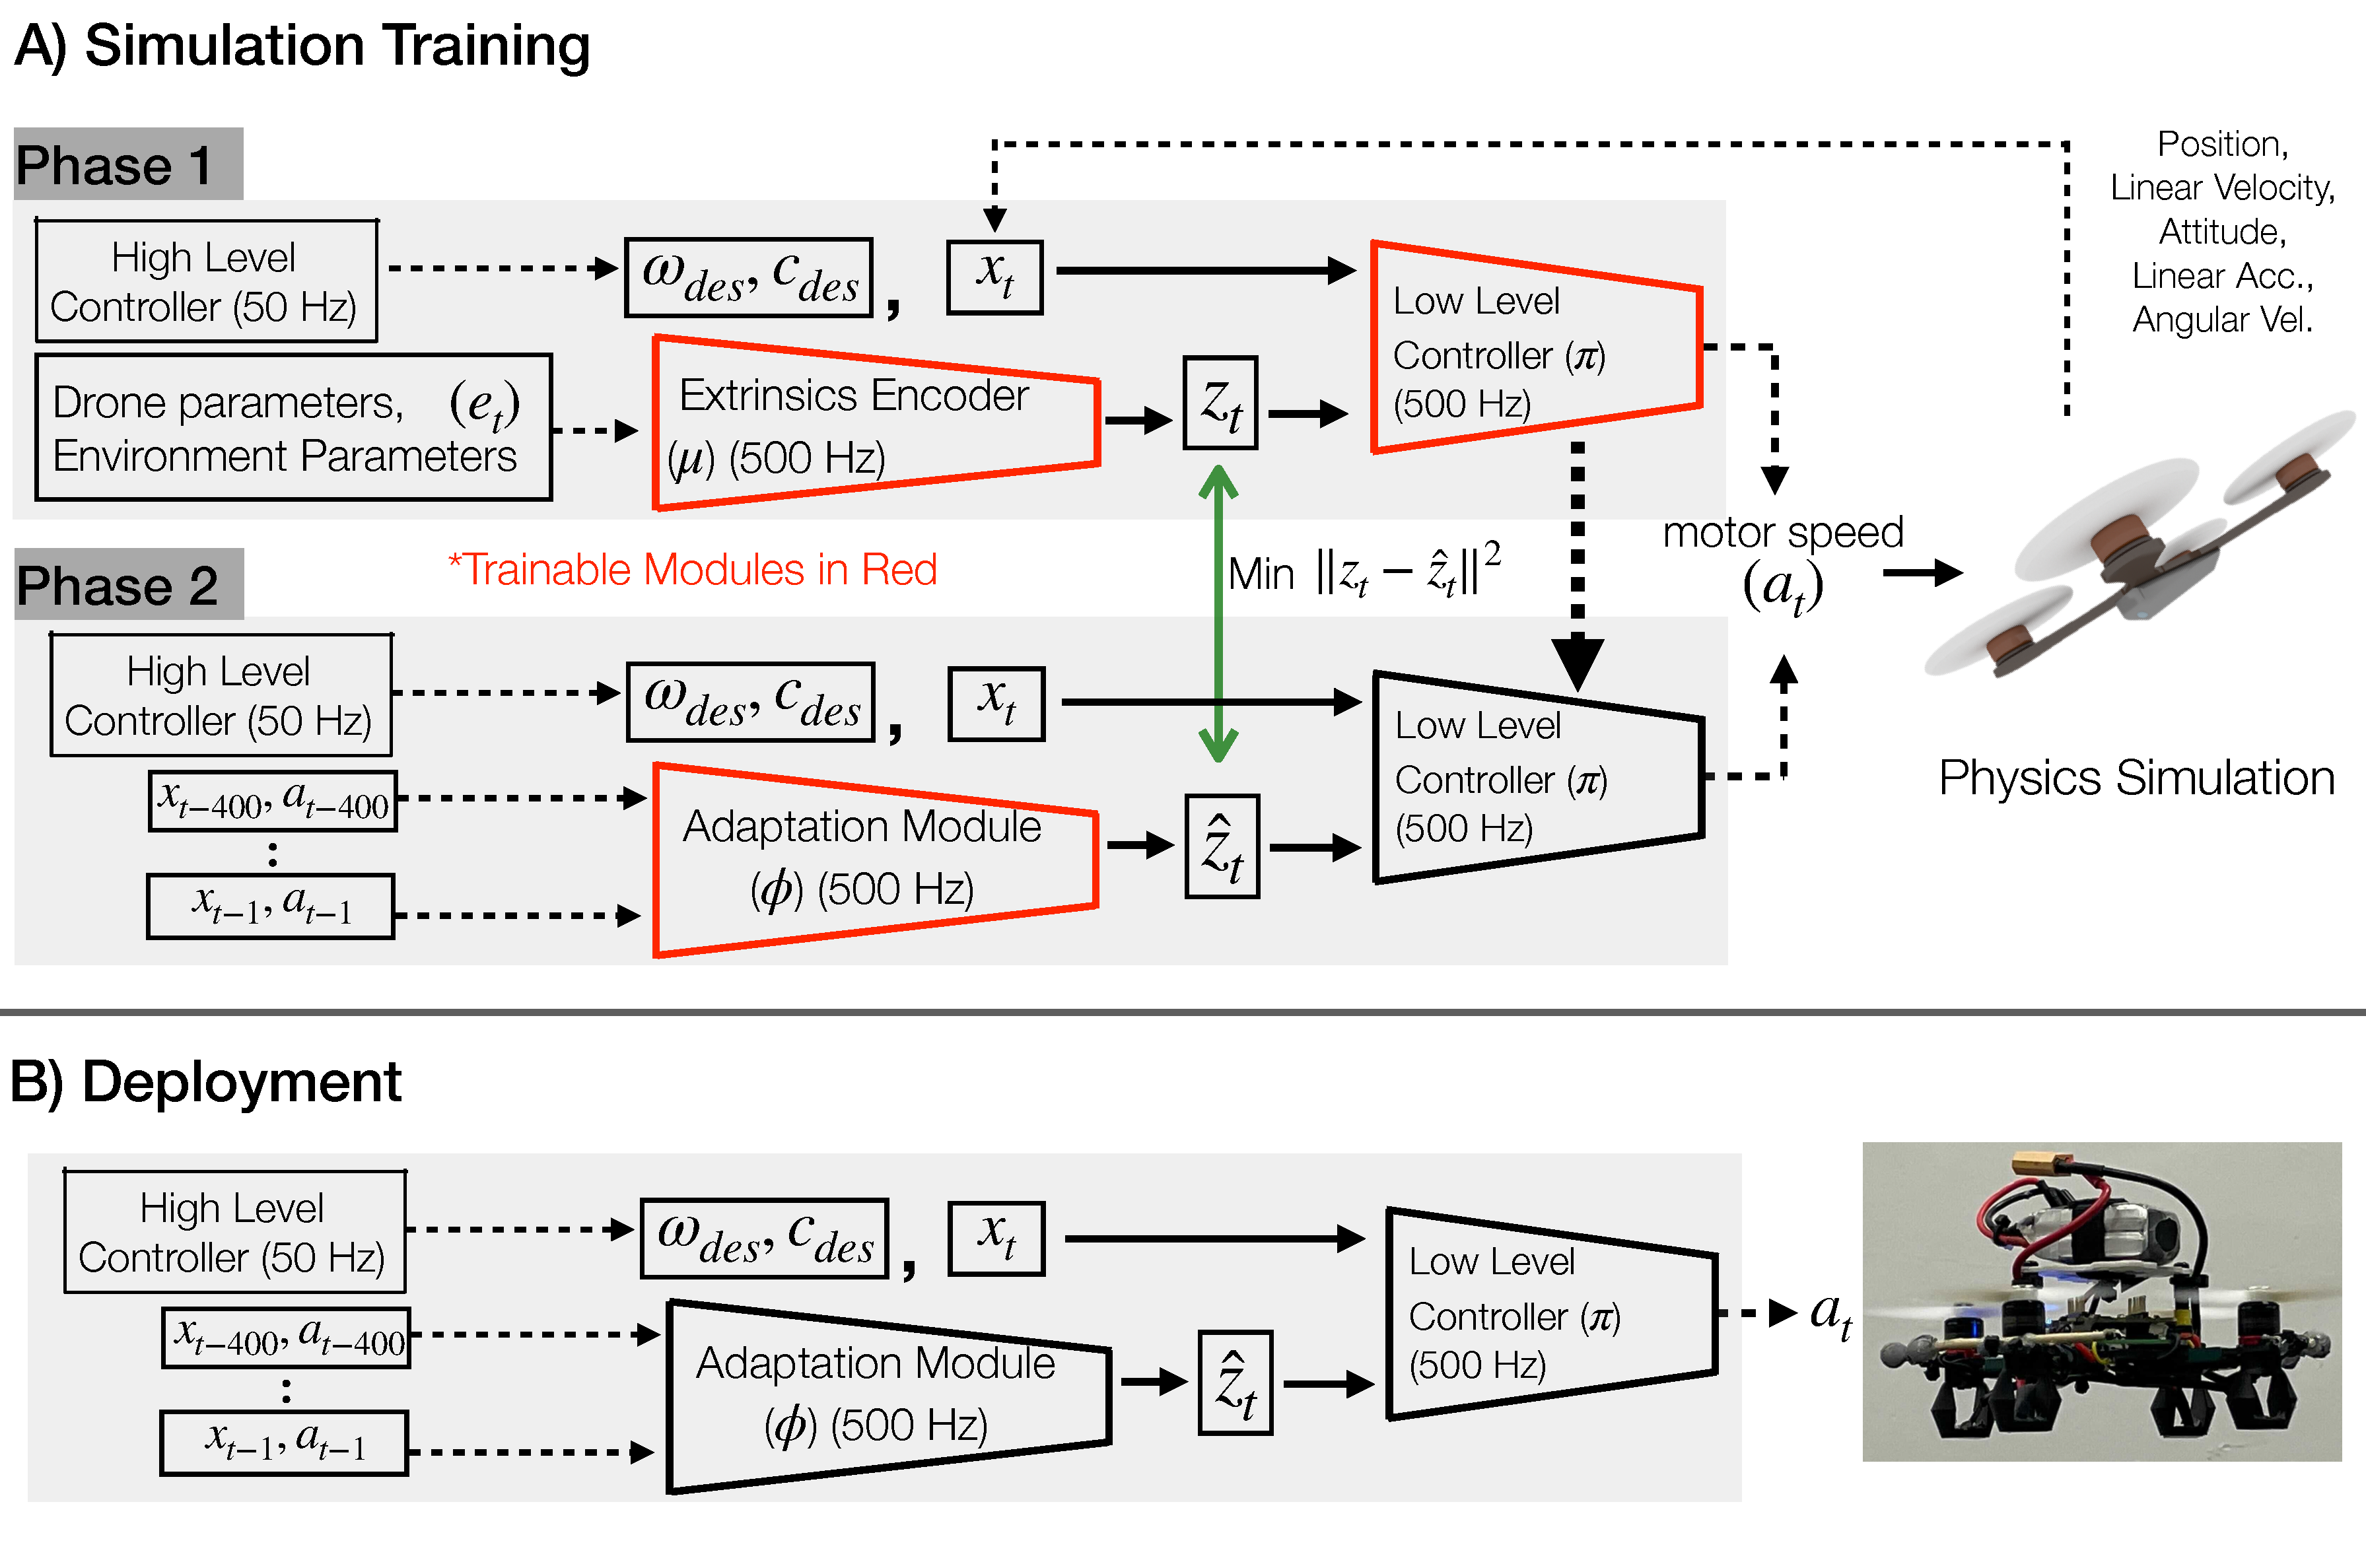
\includegraphics[width=\linewidth]{img/method-figures-no-last-act.pdf}
\caption{\small We show the training at the top and the deployment architecture of our system. We train in two phases. In the first phase, we train a base policy $\pi$ which takes the current state $x_t$, and the intrinsics vector $z_t$ which is a compressed version of the environment parameters $e_t$ generated by the module $\mu$. Since we cannot deploy this policy in the real world because we do not observe the environment parameters $e_t$, we learn an adaptation module which takes the sensor history and action history, and directly predicts the intrinsics vector $z_t$. This is done in phase two in simulation using supervised learning. We can finally deploy the base policy $\pi$ which takes as input the current state $x_t$ and the intrinsics vector $\hat{z_t}$ predicted by the adaptation module $\phi$.}
% \vspace{-5ex}
\label{fig:method}
\end{figure}

Our approach is related to existing methods in adaptive control.
%
However, our work shifts the meaning of adaptation to a different paradigm.
%
While adaptive control is generally concerned with estimating and counteracting disparities between observations and a \emph{reference} model, our approach does not have this notion. % of reference model.
%
This key difference enables adaptation to a much wider range of dynamics and disturbances.
%
In addition, it waives the engineering and tuning required by prior work when modifying the vehicle.
%
% Meta-learning is also related to the context of our problem in providing fast online adaptation.
% %
% Although they have been demonstrated on real quadcopters with impressive results on disturbance rejection~\cite{belkhale2021model,neuralfly}, they require real world learning samples to adapt.
% %
% When adapting to a much wider scale in our problem setting, this approach could be potentially dangerous for a dynamic system like a quadcopter, since failure to adapt quickly leads to catastrophic failure (a crash).
%
The closest related to our work are industrial systems like Beta-Flight~\cite{BetaFlight} and PX4~\cite{PX4}.
%
While they work well across a variety of vehicles, they still require significant in-flight tuning for each robot type and are generally tailored to human pilots.
%
% Finally, our work is also related to existing approaches in legged locomotion~\cite{kumar2021rma,lee2020learning}.
% %
% These works perform online adaptation to navigate a large variety of terrains.
% %
% However, while they adapt to different external factors (friction, terrain geometry, payload), they still rely on an accurate dynamic and morphological model of the platform \propose{to perform on one single robot}.
% %
% Therefore, changes to the robot would inevitably lead to re-training of the control policy. 
% \todo{Meta-RL}
% \propose{
% \begin{itemize}
%     \item Meta-RL is also related to our method. 
%     \item It gathers real world data to learn a latent representation of unknown disturbances or model uncertainties, then uses the learned latent to augment the base controller's performance during test time~\cite{belkhale2021model,neuralfly}
%     \item They still just perform on one platform. 
%     \item Their approach may be dangerous in our problem with the much wider range of dynamics and disturbances for dynamics systems as drones
%     \item However meta-learning could be used to complement our work in the future for a better performance 
% \end{itemize}
% }
% \begin{itemize}
%     \item Our approach is related to traditional adaptive control.
%     \item Adaptive control works well but still requires platform-specific design and tuning.
%     \item The closest related to our work are industrial systems like Beta-Flight or PX4.
%     \item They work well across vehicles, but they require tuning every time a vehicle changes.
%     \item They are also designed to work well for human pilots flight.
%     \item Our work is also related to existing approaches in legged robotics
%     \item There similar insights to ours have been used to unlock locomotion on a different set of terrains in a seamless fashion.
%     \item However, they show adaptation to different external factors (friction, terrain geometry, payload), but not to the robot body itself.
%     \item Indeed, they rely on a quite accurate system of the platform in term of platform geometry and actuation.
%     \item Some of them even rely on special purpose motor models which can only be trained with more than 30min of experience on the physical robot, and would need to be retrained any time the physical robot changes.
% \end{itemize}

% \subsection{Contributions}

% \antonio{Not really a fan of this section, would prefer to remove it}.
% We present the first universal low-level controller for quadcopters.
% %
% Our controller can cope with large variations in actuation and dynamics of the platform~\todo{quantify}.
% %
% In addition, it can react to disturbances which are difficult to model, \emph{e.g.} aerodynamics, and for which it was not explicitely trained for.
% %
% We compare our approach against baselines both in simulation and in the physical world and obtain results of up to X\% better in terms \todo{finish when we know the results}.
% %
% This work allows minimising the engineering effort required when building new platforms, potentially opening the door of drone design to a much larger audience than was previously possible.


% \begin{itemize}

%     \item We present the first universal low-level for quadcopters
%     \item It can cope with large variations in actuation and dynamics of the platform (up to 2 orders of magnitude
%     \item We compare our approach against baselines both in simulation and in the physical world and obtain results of up to X\% better in terms \todo{finish when we know the results}
%     \item This work allows to minimize the engineering effort required when building new platforms.
%     \item Easing the control problems, it potentially opens the door to a much wider space of designs and enlarges the set of people who can build drones.
    
% \end{itemize}


% \emph{What is the problem? Why is it important?}

% \emph{Why is the problem hard? What makes it challenging?}

% \emph{How far has existing work come? Why hasn't the problem been solved? What is the stumbling block? What is the frontier?}

% \emph{What does our paper contribute? What is the key idea? What is the magic trick? What is the new insight or technique that enables us to advance the frontier?}

% \emph{Any other interesting aspects of the approach or its execution?}

% \todo{Want to make sure that we emphasize that model-based control gives us very strong performance. However, creating the control requires knowledge of system parameters, like inertial parameters, motor characteristics, etc. Thus, when implementing a model-based control on a new drone, the engineer typically has to spend significant energy on estimating parameters, and tuning constants, to get the desired behaviour. Having a system that can quickly adapt to a new vehicle, and keep adapting as the vehicle's payload and environmental conditions change, would make it much easier to control a variety of vehicles with minimum engineering effort.}
\section{Related Work}
\label{sec:rel_work}

\todo{Lit Review: Should include this work ‘Hardware Conditioned
Policies for Multi-Robot Transfer Learning’ (I will refer
to this paper as [1]) . This also uses a learned latent
representation for the robot. }

% \todo{move related work ahead}
\todo{Similar feedback to the discussion: Section II.B. does not
provide a convincing argument as to why any of the existing
learning-based methods (can solve the universal control
problem). 
When comparing alternative methods, include the algorithms
used in the experimental results to strengthen the argument
as to why the universal controller has not been found yet.
}
\todo{Second of introduction should be incorporated into this
section, but otherwise the writing is clear.}

The design of high-performance adaptive controllers for aerospace systems has been a top priority for researchers and industry for more than 50 years.
% \todo{This isn't true, though? quadcopters may have been invented 100 years ago, but until we had small IMUs (maybe 20 years ago) no-one was really working on them, and certainly not a `top priority'.}
% \todo{We can maybe claim something like automatic control of aerospace systems...}
%
While the overall goal remained the same over the decades, approaches greatly evolved.
%
In the following, we review both traditional and learning-based solutions to adaptive control.
%
While each method has its advantages and limitations, they are mainly designed to handle model uncertainties and disturbances.
%
We are interested in exploring a much wider range of adaptations, with substantial differences between platforms.


\subsection{Traditional Adaptive Control}

One of the initial contributions in this space is the model reference adaptive controller (MRAC), an extension of the well-known MIT-rule~\cite{MAREELSMit}.
%
The empirical success of this method sparked great interest in the aerospace community, which led to the development of both practical tools and theoretical foundations~\cite{aastrom2013adaptive, lavretsky2013robust}.
%
From the many methods developed, one of the most popular is $\mathcal{L}1$ adaptive control~\cite{cao2008design,hovakimyan2010l1}.
%
The main reason behind its success is the ability to provide rapid adaptation to model uncertainties and disturbances with theoretical guarantees under (possibly restrictive) assumptions.
%
Its high-level working principle consists of estimating the differences between the nominal (as predicted by the reference model) and observed state transitions.
%
Such differences are then compensated by allocating a control authority proportional to the disturbance, effectively driving the system to its reference behaviour.
%
Applications of $\mathcal{L}1$ adaptive controllers span several types of aerial vehicles, from multi-rotors to fixed wings~\cite{mallikarjunan2012l1, gregory2009l1}.

Mostly related to this work is the application of $\mathcal{L}1$ adaptive control to quadcopters~\cite{schreier2012modeling}.
%
However, the performance of the classic $\mathcal{L}1$ formulation degrades whenever the observed transitions differ greatly from the (usually linear) reference model, which can happen due to aerodynamic effects or large payloads.
%
Therefore, recent work has combined $\mathcal{L}1$ adaptive control with nonlinear online optimization~\cite{hanover2021performance, pravitra2020, pereida2018adaptive}.
%
While these methods achieved impressive results, they still require explicit knowledge of (reference) system parameters, such as inertia, mass, and motor characteristics.
%
In addition, they generally require platform-specific tuning to get the desired behaviour. 
%
Other approaches to adaptive control on quadcopters include differential flatness~\cite{faessler2017differential} and nonlinear dynamic inversion~\cite{smeur2016adaptive}.
%
These methods have shown rapid adaptation to aerodynamic effects and model uncertainties.
%
However, they cannot cope with large variations in the quadcopter's dynamics, since the underlying assumptions on locally linear disturbances are generally not fulfilled.
 


%the engineer typically has to spend significant energy on estimating parameters, and tuning constants, to get the desired behaviour. 
% In quadcopters, $\mathcal{L}1$ adaptive control is generally combined with online optimization, e.g. MPC, to obtain the best performances~\cite{hanover2021performance, pravitra2020, pereida2018adaptive}.
%
% Combining $\mathcal{L}1$ adaptive control with non-linear optimization can mitigate some of these problems and achieve impressive results in high-speed flight~\cite{hanover2021performance, pravitra2020, pereida2018adaptive}.
% %
% However, they still require specific feature engineering and disturbances to be smaller in comparison to the quadcopter dynamics.
% \todo{I don't understand the previous sentence -Mark}
% \todo{There is a very abrupt jump from generic aerospace control to "quadcopter dynamics". It's also not clear what is meant by "disturbances being smaller" than "dynamics" (how do I compare them?)}

% \todo{This paragraph includes one `model learning' paper, but the next section is about learning. Is this an oversight?}
% Other approaches for adaptive control include differential flatness~\cite{faessler2017differential}, online model learning~\cite{torrente2021data}, and nonlinear dynamic inversion~\cite{smeur2016adaptive}.
% %
% These methods have shown rapid adaptation to aerodynamic effects and model uncertainties.
% %
% However, they cannot cope with large variations in the quadcopter's dynamic, since the underlying assumptions on locally linear disturbances are generally not fulfilled.
 
% \begin{itemize}
%     %\item (History) Revisiting the mit rule for adaptive control
%     %\item Performance, Precision, and Payloads: Adaptive Nonlinear MPC for quadcopters
%     %\item E. Lavretsky and K. A. Wise, “Robust adaptive control"
%     %\item K. J. Astrom and B. Wittenmark, Adaptive control.
%     %\item P. A. Ioannou and J. Sun, Robust adaptive control.
%     %\item N. Hovakimyan and C. Cao, L1 adaptive control theory: Guaranteed robustness with fast adaptation.
%     %\item  C. Cao and N. Hovakimyan, “Design and analysis of a novel l1 adaptive control architecture with guaranteed transient
%     %performance,”
%     %\item “L1 adaptive controller for attitude control of multirotors,”
%     %\item Adaptive control of quadcopter uavs: A design trade study with flight evaluations,
%     %\item Modeling and adaptive control of a quadcopter
%     %\item Geometric L1 Adaptive Attitude Control for a quadcopter Unmanned Aerial Vehicle
%     %\item "Adaptive model predictive control for high-accuracy trajectory tracking in changing conditions"
%     %\item "L1-adaptive mppi architecture for robust and agile control of multirotors,”
%     %\item Differential Flatness of quadcopter Dynamics Subject to Rotor Drag for Accurate Tracking of High-Speed Trajectories
%     %\item L1 adaptive controller for multi-input multi-output systems in the presence of nonlinear unmatched uncertainties
%     %\item Online Estimation of Geometric and Inertia Parameters for Multirotor Aerial Vehicles
%     %\item Adaptive Incremental Nonlinear Dynamic Inversion for Attitude Control of Micro Air Vehicles | Journal of Guidance, Control, and Dynamics
%     %\item Data-driven mpc for quadcopters
%     %\item IMU-Based Inertia Estimation for a quadcopter Using Newton-Euler Dynamics
%     %\item L1-RL: Robustifying Reinforcement Learning Policies with L1 Adaptive Control
% \end{itemize}

% \subsection{Robust Control}

% \begin{itemize}
%     \item “Fast direct multiple shooting algorithms for optimal robot control"
%     \item ONLINEAR ROBUST TRACKING CONTROL OF A quadcopterUADROTOR UAV ON SE(3)

% \end{itemize}

\subsection{Learning-Based Adaptive Control}

Recent data-driven controllers have shown promising results for quadcopter stabilization~\cite{hwangbo2017control,koch2019reinforcement}, or waypoint tracking flight~\cite{song2021autonomous, kaufmann2022benchmark}.
%
As their classic counterparts, learning-based controllers also allow for adaptation to disturbances and model mismatches.
%
One possibility to do so consists of learning a model from the data and using the model to adapt the controller~\cite{lambert2019low,shi2019neural,belkhale2021model,torrente2021data}.
%
However, this has the limitation that the models are difficult to carefully identify due to under-actuation of the platform and sensing noise.
%
This motivated model-free methods that, like ours, learn an end-to-end adaptive policy~\cite{pi2021robust}.
%
Meta-learning has also been proposed to augment the performance of the model-based controller for fast online adaptation to wind~\cite{neuralfly} or suspended payloads~\cite{belkhale2021model}. 
%
These methods achieved impressive results in disturbance rejection.
%
However, they are still tailored to a specific platform type, and lack an explicit mechanism for adaptation to drastic changes in the drone's model and actuation.
%
Our work aims to fill this gap and create a single control policy capable of flying vehicles with vastly varying physical characteristics and under large disturbances.
%
% However, we believe that meta-learning can complement our work on rapid adaptation by improving the policy in the real world during deployment. We will discuss this aspect in the future work and limitations section in the updated version.





% \begin{itemize}
%     %\item Model-based meta-reinforcement learning for flight with suspended payloads
%     %\item Neural lander: Stable drone landing control using learned dynamics
%     %\item Autonomous drone racing with deep reinforcement learning
%     %\item Low-level control of a quadcopter with deep model-based reinforcement learning
%     %\item Robust quadcopter control through reinforcement learning with disturbance compensation
%     %\item Low-level autonomous control and tracking of quadcopter using reinforcement learning
%     %\item Reinforcement Learning for UAV Attitude Control
%     %\item Neural-Fly enables rapid learning for agile flight in strong winds
%     %\item A Benchmark Comparison of Learned Control Policies for Agile quadcopter Flight
    
% \end{itemize}



\section{Learning a Universal Adaptive Drone Controller}
\label{sec:method}

\todo{Moving the definition intrinsics vector to the introductory
paragraph before section A will clarify your high-level
exposition before you dive into a more detailed
description.}

\todo{1. Algorithmic novelty
As far as I understand, the proposed method is an
application of RMA to the quadcopter control. Even though
the authors mention that the proposed approach "re-purpose"
the adaptation module of RMA to be suitable for the target
task, as a reviewer, it was not clear to me the mentioned
difference is significant. If the change is substantial,
clearly spelling out the difference between the proposed
method and RMA enhances the credibility of the manuscript.}

\todo{- the definition of the 23-dimensional state is not
included. }

\todo{Also, when describing the network architecture, it would be
clearer to separate better the description of the factor
encoder and the adaptation module; and give more details of
the latter for the sake of reproducibility.}

\todo{- What is the window k used in the adaptation module (it
seems the value of k is 400 according to page 4; 0.8 secs).}

We learn a universal controller to fly a quadcopter to a target position. This controller takes a history of platform states and commands from a platform-independent high level controller as inputs, and outputs individual motor speed. Our resulting policy can control quadcopters with very different design and hardware characteristics, and is robust to disturbances unseen at training time, such as swing payloads and malfunctioned motors.
%In this work, we view both of these as adaptations to parameters intrinsic and extrinsic to drones, and we will learn a single adaptive policy capable of flying multiple different quadcopter drones under variations in payload and inertia. 

 To achieve this, we use RMA~\cite{kumar2021rma}. However, we re-purpose the adaption module, originally used to estimate parameters external to the robot, e.g. friction, to estimate the robot's intrinsic parameters (e.g. its mass, inertia, motor constant, etc.) In the following, we recapitulate the method of RMA for completeness. Our policy consists of a base policy $\pi$ and an adaptation module $\phi$. The base policy $\pi$ takes the current state $x_t \in \mathbb{R}^{23}$ and an intrinsics vector $z_t \in \mathbb{R}^6$
%  which includes position (3dim), velocity (3dim), rotation(9dim), z acceleration, angular velocity (3dim) and commanded z acceleration and commanded angular velocity (3dim),
 as input and outputs the target motor speed $a_t \in \mathbb{R}^4$ for all individual motors. The intrinsics vector $z_t$ allows the base policy to adapt to variations in drone parameters, payloads, and disturbances such as wind. Since we cannot directly measure $z_t$ in the real world, we instead estimate it via the adaptation module $\phi$, which uses the discrepancy between the commanded actions and the measured sensor readings to estimate it online during deployment. More concretely, 
\begin{align}
    \hat{z_t} &=  \phi\big(x_{t-k:t-1}, a_{t-k:t-1}\big) \\
    a_t &= \pi(x_t, \hat{z_t}) \label{eq:pi}
\end{align}

\subsection{Base Policy}
We learn the base policy $\pi$ in simulation using model-free RL. The base policy takes the current state $x_t$ and the intrinsics vector $z_t$, which is a compressed version of the environment parameters $e_t$ containing drone parameters, payload, etc. We use the network $\mu$ to compress $e_t$ to $z_t$. This gives us:
\begin{align}
        z_t &= \mu(e_t) \\  
        a_t &= \pi(x_t, z_t)
\end{align}

% \todo{remove previous action from obs}

We implement $\mu$ and $\pi$ as MLPs and jointly train the base policy $\pi$ and the environmental factor encoder $\mu$ end to end using model-free reinforcement learning. RL maximizes the following expected return of the policy $\pi$: 
\begin{align}
    J(\pi) = \mathbb{E}_{\tau \sim p(\tau|\pi)}\Bigg[\sum_{t=0}^{T-1}\gamma^t r_t\Bigg],
\end{align}
where $\tau = \{(x_0, a_0, r_0), (x_1, a_1, r_1) . . .\}$ is the trajectory of the agent when executing the policy $\pi$, and $p(\tau|\pi)$ represents the likelihood of the trajectory under $\pi$.

\paragraph{RL Reward} The following reward function encourages the agent to hover at a goal position and penalizes it for crash and oscillating motions. Let us denote the acceleration in the $z$-axis i.e. the mass-normalized thrust as $\mathbf{c}$, the angular velocity as $\bm{\omega}$, all in the quadcopter's body frame. The commanded mass-normalized thrust is defined as $\bm{c}_{des}$, commanded angular velocity as $\bm{\omega}_{des}$, all given by the high-level controller.
We additionally define the motor speed as $\bm{m}$ and the simulation step in the training as $\bm{\delta t}$. The reward at time $t$ is defined as the sum of the following quantities:
\begin{enumerate}
    \item Angular Velocity Tracking : $-\| \bm{\omega}^{t} - \bm{\omega}_{des}^{t} \|$
    \item Z Acceleration Tracking: $-\| \mathbf{c}^{t} - \mathbf{c}_{des}^{t} \|$
    \item Output Command Smoothness: $-\| \bm{m}^{t} - \bm{m}^{t-1} \|$
    \item Survive: $\bm{\delta t}$
\end{enumerate}
The scaling factor of each reward term is $0.01$, $0.02$, $0.0002$, $1$ respectively. 

  
\begin{table}[t]
\setlength{\tabcolsep}{5.5pt}
\begin{center}
\begin{tabular}{lcc}
\toprule
 \textbf{Parameters} & \textbf{Training Range} & \textbf{Testing Range} \\
 \midrule
 Mass (kg) & [0.142, 0.950]  & [0.114, 1.140]  \\
 Arm length (m) & [0.046, 0.200] & [[0.037, 0.240] \\
 Mass moment of inertia  & \multirow{2}{*}{ [7.42e-5 , 5.60e-3]}&\multirow{2}{*}{ [5.94e-5 , 6.72e-3]} \\
%  [7.42e-5 , 5.60e-3 ] & [5.94e-5 , 6.72e-3 ]   \\
 around $x$, $y$ (kg$\cdot$m$^2$)&&\\
  Mass moment of inertia  & \multirow{2}{*}{[1.20e-4, 8.80e-3]} &  \multirow{2}{*}{[9.60e-5, 1.06e-2]} \\
  around $z$ (kg$\cdot$m$^2$)&&\\
 Propeller constant $\kappa$ (m) & [0.0041, 0.0168] & [0.0033, 0.0201]\\
 Payload (\% of Mass)  & [10, 50] & [5, 60] \\
 Payload Location & \multirow{3}{*}{[-10, 10]}  & \multirow{3}{*}{[-10, 10]}  \\
 from Center of Mass&&\\
 (\% of Arm length)&&\\
 Motor Constant & [1.15e-7, 7.64e-6] & [9.16e-8, 9.17e-6]  \\
 Body drag coefficient & [0, 0.62]& [0, 0.74] \\
 Max. motor speed (rad/s) & [707, 4895] & [566, 5874] \\
\bottomrule
\end{tabular}
\vspace{1ex}
\caption{\label{tab:randomization} Ranges of the drone and environmental parameters. Parameters without units labelled are dimensionless quantities.}
% \marksez{$\kappa$ has units too, if it is "propellerTorqueFromThrust" from our lab sim code, the units are [m]. If it is really `torque to thrust' as in the paper, its units are [1/m].}
\end{center}
\end{table}


% \paragraph{Drone and Environment Randomization} We randomize the drone parameters which includes mass, arm length, inertia matrix, $\kappa$ ( propeller torque to thrust ratio constant), propeller thrust from speed squared constant, body drag coefficient, max motor speed and other external parameters like payload (Table~\ref{tab:randomization}). Note that we define a single vector $e_t$ which includes both the drone and the environment parameters and compress it into a single extrinsics vector $z_t$.  

\subsection{Adaptation Module}
During deployment, we do not have access to the vector $e_t$ and hence we cannot compute the intrinsics vector $z$. Instead, we will use the sensor and action history to directly estimate $z_t$ as proposed in ~\cite{kumar2021rma}. We call this module the adaptation module $\phi$, and we will train this in simulation itself $a_t = \pi(x_t, \hat{z_t})$. We can train this module in simulation using supervised learning because we have access to both the ground truth intrinsics $z_t$, and the sensor history and previous actions. We minimize the mean squared error loss $\lVert z - \hat{z} \rVert ^2$.  

\subsection{Deployment}
We directly deploy the base policy $\pi$ which uses the current state and the intrinsics vector $\hat{z}$ predicted by the adaptation module $\phi$. We do not calibrate or finetune our policy on any drones and use the same policy without any modifications as the controller of the different drones under different payload and conditions.
\section{Experimental Setup}

\mypara{Simulation Environment} We use the Flightmare simulator~\cite{song2020flightmare} for training and testing our control policies. 
We implement a custom high-level controller to generates high-level commands at the level of body rates and collective thrust.
It is designed as a cascaded linear acceleration controller (with desired acceleration mimicking a spring-mass-damper system with natural frequency 2rad/s and damping ratio 0.7. The desired acceleration is then converted to a desired total thrust and the desired thrust direction, and the body rates are computed from this as proportional to the attitude error angle, with a time constant of 0.2s.
% \marksez{The gains are a little hard to express compactly here. The rates are computed as (ignoring the nonlinear aspects) proportional to position, velocity, and angle error. I.e., the command has a "P" term, a "D" term, and a "double-D" term (as angle is like acceleration, to first order). 
% % Can perhaps describe it as follows:
% `We implement a custom high-level controller, that is designed as a cascaded linear acceleration controller (with desired acceleration mimicking a spring-mass-damper system with natural frequency 2rad/s and damping ratio 0.7. The desired acceleration is then converted to a desired total thrust, and desired thrust direction, and body rates are computed from this as proportional to the attitude error angle, with time constant 0.2s.'
% }
%
We define the task as hovering at a pre-defined location.
%
This high-level controller's inputs are the platform's state (position, rotation, angular, and linear velocities) and the goal location. 
%
The policy outputs individual motor speed commands, and we model the motors' response using a first-order system.
% We train the policy with model-free RL, using the PPO algorithm~\cite{schulman2017proximal}.
%
Each RL episode lasts for a maximum of 5s of simulated time, with early termination if the quadcopter height drops below 2cm.
%
The control frequency of the policy is $500$Hz, and the simulation step is 2ms.
%
We additionally implement an observation latency of 10ms.

\mypara{Quadcopter and Environment Randomization} All our training and testing ranges are listed in Table~\ref{tab:randomization}. Of these, $e_t$ includes mass, arm length, propeller torque to thrust ratio $\kappa$, motor constant, inertia (9dim), body drag coefficients (3dim), maximum motor rotation and payload mass, which results in an 18-dim vector.
%
We randomize each of these parameters at the end of each episode. In addition, at a randomly sampled time during each episode, the parameters including mass, inertia, and the Center of Mass are also randomized. 
% \marksez{What does it mean to randomize at the end of an episode? Do we mean at the beginning of each episode? Isn't everything discarded at the end?}
%
The latter is used to mimic sudden variations in the quadcopter parameters due to a sudden disturbance caused by a payload or wind.



\mypara{Hardware Details} For all our real-world experiments we use two quadcopters, which differ in mass by a factor of 4.5, and in size by a factor of 2.9. 
The first one, which we name \emph{largequad} has a mass of 792g, a size of 16.6cm in arm length, a thrust-to-weight ratio of 3.50, a diagonal inertia matrix of [0.0047, 0.005, 0.0074]kg$\cdot$m$^2$ (as expressed in the z-up body-fixed frame), and a maximum motor speed of 943rad/s. The second one, \emph{miniquad}, has a mass of 177g, a size of 5.8cm in arm length, a thrust-to-weight ratio of 3.45, a diagonal inertia matrix of [92.7e-6, 92.7e-6, 158.57e-6]kg$\cdot$m$^2$, and a maximum motor speed of 3916rad/s.
%
A motion capture system running at $200$Hz provides estimates of the drone position and orientation, which is followed by a Kalman filter to reduce noise and estimate linear velocity.
%
An onboard rate gyroscope measures the angular rotation of the robot, which is low-pass filtered to reduce noise and remove outliers.
%
The deployed policy outputs motor speed commands, which are subsequently tracked by off-the-shelf electronic speed controllers.
%
We use as high-level a PD controller which takes as input the goal position and outputs the mass normalized collective trust and the body rates.

\mypara{Network Architecture and Training Procedure} The base policy is a 3-layer Multi-layer perceptron (MLP) with 256-dim hidden layers. This takes the drone state and the vector of intrinsics as input to produce motor speeds. The environment factor encoder is a 2-layer MLP with 128-dim hidden layers.  The policy and the value function share the same factor encoding layer. The adaptation module projects the latest 400 state-action pairs into a 128-dim representation. Then, a 3-layer 1-D CNN convolves the representation across time. The flattened CNN output is linearly projected to estimate $z_t$. We train the base policy and the environment encoder using PPO~\cite{schulman2017proximal} for 100M steps. We use the reward outlined in Section~\ref{sec:method}. Policy training takes approximately 2 hours on an ordinary desktop machine with 1 GPU.
%
We finally train the adaptation module with supervised learning by rolling out the student policy. We train with the ADAM optimizer to minimize MSE loss. 
%
We run the optimization process for 10M steps, training on data collected over the last 1M steps. Training the adaptation module takes approximately 20 minutes.



\section{Results}

% \begin{figure}[t]
%     \centering
%     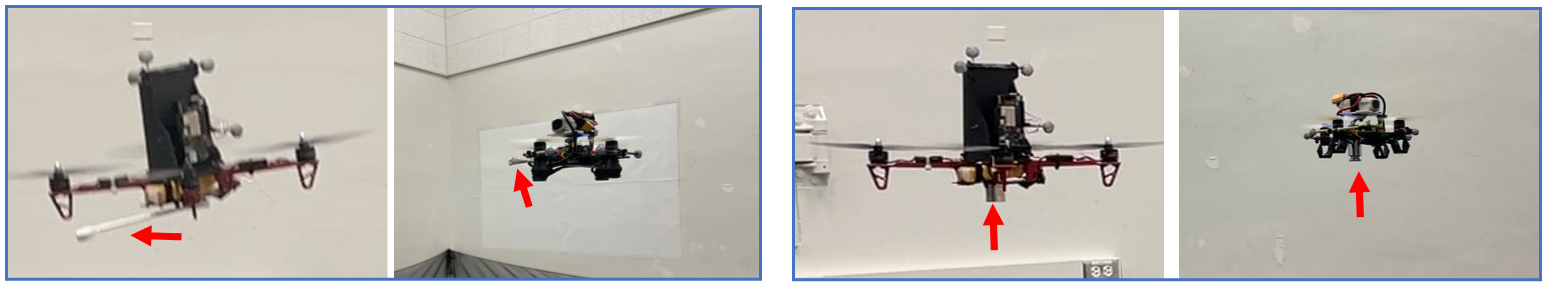
\includegraphics[width=\linewidth]{img/Disturbances_2.png}
%     \caption{\textbf{Left}: Large and small quadcopters mounted with an inertia board. For the large quadcopter, we mount a wrench of 20.5cm and 140g. For the small quadcopter, a wrench of 14.5cm and 30g. \textbf{Right}: Large and small quadcopters with a rigid payload. For the former, we add a load of 180g ($\approx 25\%$ of its weight). For the latter, we add a load of 50g, which corresponds to 35.7\% of its weight. Despite such large disturbances unknown to the control policy, our approach can always stabilize the quadcopter. Videos at~\url{https://dz298.github.io/universal-drone-controller/}}
%     \label{fig:distur}
% \end{figure}

\begin{figure}[t]
    \centering
    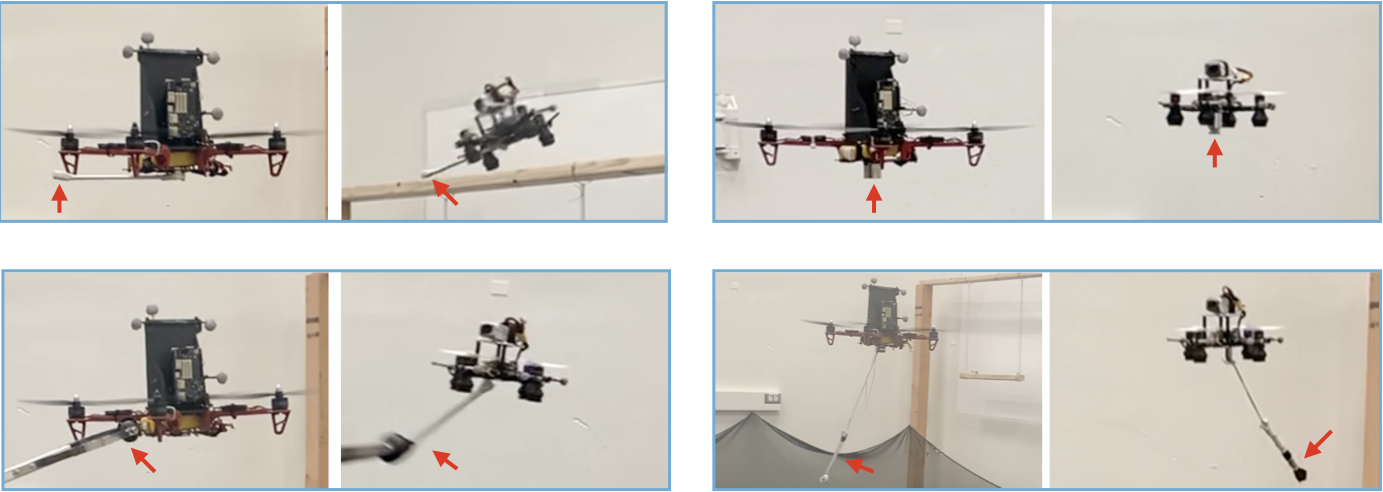
\includegraphics[width=\linewidth]{img/disturbance-include-held-out.png}
    \caption{\textbf{Upper Left}: Large and small quadcopters mounted with an inertia board. For the large quadcopter, we mount a wrench of 20.5cm and 140g. For the small quadcopter, a wrench of 14.5cm and 30g. \textbf{Upper Right}: Large and small quadcopters with a rigid payload. For the former, we add a load of 180g ($\approx 25\%$ of its weight). For the latter, we add a load of 50g, which corresponds to 35.7\% of its weight. \textbf{Lower Left}: Large and small quadcopters with random pushes/pulls. \textbf{Lower Right}: Large and small quadcopters with a swing payload, which is the wrench in the inertia board test. Despite such large disturbances unknown to the control policy, our approach can always stabilize the quadcopter.}
    \label{fig:distur}
\end{figure}

% Please add the following required packages to your document preamble:
% \usepackage{multirow}
% \begin{table}[t]
% \def \arraystretch{1.2}
% \centering
% % \caption{Experimental results.}
% % \label{tab:experimental_result.}
% \begin{tabular}{|l|l|l|l|l|l|}
% \hline
%  & vehicle & method & \begin{tabular}[c]{@{}l@{}}Avg. Err. \\ in height {[}m{]}\end{tabular} & \begin{tabular}[c]{@{}l@{}}Avg.  Err. \\ ang. vel. {[}rad/s{]}\end{tabular} & \begin{tabular}[c]{@{}l@{}}Avg. Err. \\ normalized thrust {[}m/s$^2${]}\end{tabular} \\ \hline
% \multirow{4}{*}{\begin{tabular}[c]{@{}l@{}}Inertial \\ board\end{tabular}} & \multirow{2}{*}{large} & PD & 0.492 & 1.347 & 1.519 \\ \cline{3-6} 
%  &  & Ours & 0.061 & 2.257 & 0.277 \\ \cline{2-6} 
%  & \multirow{2}{*}{small} & PD & 0.391 & 2.477 & 1.436 \\ \cline{3-6} 
%  &  & Ours & 0.250 & 2.351 & 0.761 \\ \hline
% \multicolumn{1}{|c|}{\multirow{4}{*}{Payload}} & \multirow{2}{*}{large} & PD & 0.617 & 0.404 & 1.744 \\ \cline{3-6} 
% \multicolumn{1}{|c|}{} &  & Ours & 0.038 & 1.251 & 0.037 \\ \cline{2-6} 
% \multicolumn{1}{|c|}{} & \multirow{2}{*}{small} & PD & 0.185 & 1.548 & 1.670 \\ \cline{3-6} 
% \multicolumn{1}{|c|}{} &  & Ours & 0.182 & 1.835 & 0.902 \\ \hline
% \end{tabular}
% \vspace{2ex}
% \caption{\label{tab:rw_results} \textbf{Real-World  Results.} We compare the performance of our controller to the PID controller which has specifically been tuned to the two quadcopters with in-flight tests. We see that our approach significantly outperforms the PD baseline in terms of average height error and tracking error on the applied thrust. The two methods perform similarly on angular velocity tracking with the PD controller sometimes outperforming our method. This is expected because our reward function favours safety over tracking performance by having a large penalty on crashing. Metrics are averaged over 5 experiments.}
% \end{table}


\begin{table}[t]
\setlength{\tabcolsep}{3pt}
\def \arraystretch{1.4}
\centering
% \caption{Experimental results.}
% \label{tab:experimental_result.}
\begin{tabular}{lllllll}
\toprule
%   \multirow{2}{*}{\textbf{External Forces}} & Success & Height  & Ang. Vel. &  Thrust \\ &Rate& Err. (m) &Err. (rad/s)  & Err. (m/s$^2$) \\%& Learning Samples\\ 
 & \multirow{2}{*}{Vehicle}& \multirow{2}{*}{Method}& Height & Ang. Vel. & Thrust& Success\\&&&Err. (m)&Err. (rad/s)&Err. (m/s$^2$)& Rate\\
\midrule
\multirow{6}{*}{\begin{tabular}[c]{@{}l@{}}\textbf{Free} \\ \textbf{Hover}\end{tabular}} & \multirow{3}{*}{small} & PID & 0.06 & 0.51 & 0.57 &  100\\ %\cline{3-6} 
&  & LTF~\cite{LTF} & 0.09 & 0.78 & 0.78 & 80 \\
 &  & Ours & 0.05 & 0.30 & 0.30 & 100 \\ \cline{2-7} 
 & \multirow{3}{*}{large} & PID & 0.01 & 0.12 & 0.28 & 100 \\ %\cline{3-6} 
 &  & LTF~\cite{LTF} & 0.03 & 1.21 & 1.86 & 80 \\
 &  & Ours & 0.03 & 0.19 & 0.36 & 100 \\ \midrule
 
 
 
\multirow{6}{*}{\begin{tabular}[c]{@{}l@{}}\textbf{Inertial} \\ \textbf{Board}\end{tabular}} & \multirow{3}{*}{small} & PID & - & - & - &  0\\ %\cline{3-6} 
&  & LTF~\cite{LTF} & - & - & - & 0 \\
 &  & Ours & 0.08 & 1.14 & 1.09 & 100 \\ \cline{2-7} 
 & \multirow{3}{*}{large} & PID & 0.31 & 0.37 & 1.46 & 100 \\ %\cline{3-6} 
 &  & LTF~\cite{LTF} & - & - & - & 0 \\
 &  & Ours & 0.08 & 0.24 & 1.35 & 100 \\ \midrule
 
 
 
\multicolumn{1}{c}{\multirow{6}{*}{\textbf{Payload}}} & \multirow{3}{*}{small} & PID & 0.40 & 1.14 & 2.20 & 80 \\ %\cline{3-6} 
&  & LTF~\cite{LTF} & 0.10 & 0.98 & 2.14 & 100 \\
\multicolumn{1}{c}{} &  & Ours & 0.05 & 0.88 & 0.51 & 100 \\ \cline{2-7} 
\multicolumn{1}{c}{} & \multirow{2}{*}{large} & PID & 0.19 & 1.14 & 1.21 & 100 \\ %\cline{3-6} 
&  & LTF~\cite{LTF} & 0.06 & 1.01 & 4.2 & 100 \\
\multicolumn{1}{c}{} &  & Ours & 0.04 & 0.34 & 1.19 & 100 \\
\bottomrule
\end{tabular}
\vspace{2ex}
\caption{\label{tab:rw_results} \textbf{Real-World  Results:} We compare the performance of our controller to two baselines: \emph{LTF} and a PID controller. The comparison is run on three tasks for large and small quadcopters. \textbf{Free Hover}: hover at the goal position without any disturbances. \textbf{Inertia Board}: hover at the goal position under an unknown mass and inertia disturbance. \textbf{Payload}: hover at the goal position under an unknown mass disturbance.  
% The \emph{LTF} learns a robust policy to all variations seen in the training by inputting an error integration into observations, while the PID controller has specifically been tuned to the two quadcopters with in-flight tests. We see that our approach significantly outperforms the two baseline in all metrics under all disturbances, particularly in inertia board case. Our method and the PID controller perform similarly on free hovering case with the PID controller sometimes outperforming our method. This is expected because the PID controller is specifically tuned for each quadcopter. 
Metrics are averaged over 5 experiments.}
\end{table}



\subsection{Real World Deployment}

We test our approach in the physical world and compare its performance to two baselines: \emph{LTF}, which is a learning-based robust controller trained with an error integration as one of inputs~\cite{LTF}; and a platform-specific PID controller.
%
The PID controller has access to the platform's mass and inertia, and it has been specifically tuned to the platform with in-flight tests.
%
In contrast, our approach has no knowledge whatsoever of the physical characteristics of the system and requires no calibration or real-world fine tuning.
%
We compare the task of stabilization to a predefined set point without any disturbances (free hover), or under an unknown mass and/or inertia disturbance (Figure~\ref{fig:distur}).
%
We compare the three approaches under four metrics: (i) the average height error to the goal point, and the average tracking error of the (ii) angular velocity and (iii) mass normalized thrust of the high-level controller's commands, and the success rate.
%
We define a failure if the human operator had to intervene to avoid the quadcopter from crashing.
%
The results of these experiments are reported in table~\ref{tab:rw_results}.
%
Our approach significantly outperforms both baselines in all metrics under all disturbances. In particular, our approach achieves a 100\% success rate when asymmetric disturbances are applied to the system, while the two baselines both experience at least one total failure on either of the two platforms. 
%
The PID baseline and our approach performs similarly in free hovering experiment, with the PID controller slightly outperforming ours on \emph{largequad}.  
%
The latter difference in performance is justified, since the PID controller is specifically tuned for each quadcopter, but ours does not have knowledge of the system dynamics and hardware. 
%
% Our approach significantly outperforms the PD baseline and the LTF baseline in all metrics. in terms of success rate, average height error, and tracking error on the applied thrust.
%
% The two methods perform similarly on tracking the angular velocity commands, with the PD slightly outperforming ours in some of the tests.
%
%However, our approach significantly outperforms the PD baseline in terms of average height error and tracking error on the applied thrust.
%
% The latter difference in performance is justified by the training procedure of our controller, which favours safety to tracking performance.
%
%Indeed, we strongly penalize the agent at training time for losing height or crashing into the ground.


\subsection{Simulation Results}

% \begin{table*}[t]
% \begin{center}
% \begin{tabular*}{0.95\textwidth}{@{}lcccc@{}}
% \toprule
%   & Success Rate & Avg. Err.  & Avg.  Err. &  Avg. Err. \\ && in height [m] &ang. vel. [rad/s]  & normalized thrust \\%& Learning Samples\\ 
% \midrule
%  Robust~\cite{peng2018sim,tobin2017domain} & 4\%& 18.50 & 6.06 & 15.15 \\ 
%  SysID~\cite{SysID} & 54\%& 0.33 & 1.88 & 2.43\\
%  Ours & 64\% & 0.24 & 1.76 & 2.84 \\
% \bottomrule
% \end{tabular*}
% \caption{\label{tab:sim-metrics} \textbf{Simulation Testing Results:} We compare our method which uses adaptation in the extrinsics space, to two baselines: \emph{Robust} and \emph{SysID}. The \emph{Robust} learns a single conservative flying method for all the variations seen during training, while the \emph{SysID} baseline tries to predict the exact environment parameters which is both not difficult and not necessary to solve the task. We observe that our method which is adaptive and estimates a low dimensional extrinsics out performs both the baselines on the success rate and the average height tracking error. Because of the higher success rate, our method has to solve additional scenarios which are potentially more challenging, which explains the lower tracking error on one of the metrics. Metrics are averages over 100 experiments. 
% \vspace{-3ex}
% }
% \end{center}
% \end{table*}

\begin{table}[h]
\centering
\begin{tabular*}{0.45\textwidth}{@{}lcccc@{}}
\toprule
   & Success & Height  & Ang. Vel. &  Thrust \\ &Rate& Err. (m) &Err. (rad/s)  & Err. (m/s$^2$) \\%& Learning Samples\\ 
\midrule
 Robust~\cite{peng2018sim,tobin2017domain} & 18\%& 0.44 & 1.32 & 1.93 \\ 
 SysID~\cite{SysID} & 38\%& 0.19 & 1.10 & 1.38\\
 LTF~\cite{LTF} & 59\% & 0.35 & 0.97 & 1.68 \\
 $\mathcal{L}1$~\cite{hanover2021performance} & 59\% & 0.17 & 0.92 & 1.60 \\
 Ours & 66\% & 0.09 & 0.94 & 1.57 \\
 \midrule
 Expert (Phase I) & 69\% & 0.09 & 0.91 & 1.29 \\
\bottomrule
\end{tabular*}
% \begin{tabular}{cccccc}
% \toprule
%               & Robust & SysID & LTF     & L1   & Ours \\
%               \midrule
% success rate  & 18\%   & 38\%  & 59\% & 59\% & 66\% \\
% \midrule
% posx err      & 0.23   & 0.07  & 0.04    & 0.01 & 0.05 \\
% posy err      & 0.14   & 0.06  & 0.09    & 0.01 & 0.18 \\
% posz err      & 0.44   & 0.19  & 0.35    & 0.17 & 0.09 \\
% \midrule
% velx err      & 0.09   & 0.08  & 0.09    & 0.11 & 0.04 \\
% vely err      & 0.10   & 0.02  & 0.14    & 0.11 & 0.12 \\
% velz err      & 0.14   & 0.07  & 0.16    & 0.16 & 0.08 \\
% \midrule
% thrust err    & 1.93   & 1.38  & 1.68    & 1.60 & 1.57 \\
% ang vel z err & 1.65   & 0.89  & 0.72    & 0.21 & 0.78 \\
% ang vel x err & 1.15   & 1.35  & 1.09    & 1.28 & 0.93 \\
% ang vel y err & 1.16   & 1.06  & 1.10    & 1.25 & 1.09 \\
% \bottomrule
% \end{tabular}
\caption{\label{tab:sim-metrics} \textbf{Simulation Testing Results:} We compare our method with four baselines on the task of stabilization: \emph{Robust}, \emph{SysID}, \emph{LTF}, and $\mathcal{L}1$. We also list the results of our method in Phase I training, which has access to all ground-truth system parameters and can be regarded as the expert. The test ranges are defined in Table~\ref{tab:randomization}.
% The \emph{Robust} learns a single conservative flying method for all the variations seen during training; the \emph{SysID} baseline tries to predict the exact environment parameters which is both not difficult and not necessary to solve the task; the \emph{LTF} baseline learns a robust policy with an additional input of an error integration; and the $\mathcal{L}1$ is a model-based adaptive controller which estimates and compensates for difference between the nominal and observed states. We observe that our method which is adaptive and estimates a low dimensional intrinsics outperforms all the baselines on the success rate and the average height tracking error. Our method also achieves comparable performance on the tracking of average angular velocity and normalized thrust with baselines best on these metrics. Our method's performance is most closest to the performance of the expert Phase I which has access to the ground truth system parameters. 
Metrics are averages over 100 experiments.
\vspace{-3ex}
}
\end{table}

\begin{table}[h]
\centering
\begin{tabular*}{0.45\textwidth}{@{}lcccc@{}}
\toprule
  \multirow{2}{*}{\textbf{External Forces}} & Success & Height  & Ang. Vel. &  Thrust \\ &Rate& Err. (m) &Err. (rad/s)  & Err. (m/s$^2$) \\%& Learning Samples\\ 
\midrule
 Robust~\cite{peng2018sim,tobin2017domain} & 5\%& 0.39 & 2.05 & 1.51 \\ 
 SysID~\cite{SysID} & 2\%& 0.22 & 1.38 & 1.23\\
 LTF~\cite{LTF} & 32\% & 0.23 & 1.53 & 0.99 \\
 $\mathcal{L}1$~\cite{hanover2021performance} & 42\% & 0.30 & 1.46 & 1.04 \\
 Ours & 49\% & 0.09 & 1.40 & 0.85\\
 \midrule
 \multicolumn{2}{@{}l}{\textbf{Partially Failing Motors}} &&& \\
 Robust~\cite{peng2018sim,tobin2017domain} & 1\%& 0.53 & 1.94 & 1.59 \\ 
 SysID~\cite{SysID} & 14\%& 0.33 & 1.25 & 1.23\\
 LTF~\cite{LTF} & 21\% & 0.38 & 1.57 & 1.35 \\
 $\mathcal{L}1$~\cite{hanover2021performance} & 33\% & 0.32 & 1.41 & 1.06 \\
 Ours & 38\% & 0.26 & 1.36 & 1.01\\
\bottomrule
\end{tabular*}
\caption{\label{tab:sim-metrics-unseen-disturb} \textbf{Simulation Testing Results, Out-of-Distribution Disturbances}: We evaluate the performance of our method and all baselines on two types of disturbances unseen at training time. \textbf{External Forces}: We apply a random force of magnitude uniformly sampled between 0 and 50\% of the weight and with direction uniformly sampled on a cube. \textbf{Partially Failing Motors}: To simulate a motor losing efficiency, we multiply the output of a randomly sampled motor’s thrust force to a random number between 0 and 1. The duration of each disturbance is random between the entire length of the episode (on and off with 2\% probability at every time stamp).
\vspace{-3ex}
}
\end{table}

% \begin{table*}[h]
% \centering
% \begin{tabular}{lrrrrr}
% \toprule
%                 & \multicolumn{1}{l}{SysID} & \multicolumn{1}{l}{Robust} & \multicolumn{1}{l}{LTF} & \multicolumn{1}{l}{L1}   & \multicolumn{1}{l}{Ours} \\
%                 \midrule
% success rate    & 2\%                        & 5\%                         & 32\%                     & 42\%                      & 49\%    \\
% \midrule
% posx err        & 0.43                      & 0.73                       & 0.32                    & 0.91                     & 0.32                     \\
% posy err        & 0.53                      & 0.47                       & 0.30                    & 0.92                     & 0.34                     \\
% posz err        & 0.22                      & 0.39                       & 0.23                    & 0.30                     & 0.09                     \\
% \midrule
% velx err        & 0.43                      & 0.40                       & 0.31                    & 0.30                     & 0.31                     \\
% vely err        & 0.44                      & 0.45                       & 0.29                    & 0.22                     & 0.24                     \\
% velz err        & 0.08                      & 0.13                       & 0.07                    & 0.13                     & 0.05                     \\
% \midrule
% thrust err      & 1.38                      & 2.05                       & 1.53                    & 1.46                     & 1.40                     \\
% ang vel z err   & 0.92                      & 1.63                       & 0.71                    & 0.22                     & 0.69                     \\
% ang vel x err   & 1.73                      & 1.52                       & 1.13                    & 1.45                     & 0.85                     \\
% ang vel y err   & 1.05                      & 1.36                       & 1.12                    & 1.45                     & 0.99                     \\
% \bottomrule
% \end{tabular}
% \caption{\label{tab:sim-metrics-ext-force} \textbf{Simulation Results, External Forces:}  We apply a random force of magnitude uniformly sampled between 0 and 50\% of the weight and with direction uniformly sampled on a cube. The duration is random between the entire length of the episode (on and off with 2\% probability at every time stamp).
% \vspace{-3ex}}
% \end{table*}


% \begin{table*}[h]
% \centering
% \begin{tabular}{lrrrrr}
% \toprule
%               & \multicolumn{1}{l}{Robust} & \multicolumn{1}{l}{SysID} & \multicolumn{1}{l}{LTF} & \multicolumn{1}{l}{L1} & \multicolumn{1}{l}{Ours} \\
%               \midrule
% success rate  & 1\%                        & 14\%                      & 21\%                    & 33\%                   & 38\%                     \\
% \midrule
% posx err      & 0.39                       & 0.16                      & 0.44                    & 0.10                   & 0.15                     \\
% posy err      & 0.32                       & 0.13                      & 0.20                    & 0.10                   & 0.13                     \\
% posz err      & 0.53                       & 0.33                      & 0.38                    & 0.32                   & 0.26                     \\
% \midrule
% velx err      & 0.44                       & 0.45                      & 0.53                    & 0.20                   & 0.22                     \\
% vely err      & 0.36                       & 0.19                      & 0.20                    & 0.19                   & 0.16                     \\
% velz err      & 0.61                       & 0.85                      & 1.14                    & 0.79                   & 0.90                     \\
% \midrule
% thrust err    & 1.94                       & 1.25                      & 1.57                    & 1.41                   & 1.36                     \\
% ang vel z err & 1.62                       & 0.91                      & 0.81                    & 0.23                   & 0.63               \\
% ang vel x err & 1.53                       & 1.53                      & 1.62                    & 1.48                   & 1.13                     \\
% ang vel y err & 1.63                       & 1.26                      & 1.63                    & 1.47                   & 1.26                     \\
% \bottomrule
% \end{tabular}
% \caption{\label{tab:sim-metrics-partial-motor-fail} \textbf{Simulation Results, Partially Failing Motors:}  To simulate a motor losing efficiency, we multiply the output of a randomly sampled motor’s thrust force to a random number between 0 and 1. 
% \vspace{-3ex}}
% \end{table*}



Finally, we compare our approach with a set of baselines in the simulation.
%
We select four baselines from prior work: \emph{Robust}, which consists of a policy trained without access to environment factors or body parameters~\cite{tobin2017domain, peng2018sim}; \emph{SysID}, which directly predicts the ground-truth parameters $e_t$~\cite{SysID} instead of the low-dimensional intrinsics vector; \emph{LTF}, which essentially is a robust policy with an error integration as additional inputs~\cite{LTF}; and $\mathcal{L}1$, a model-based adaptive controller which estimates and compensates the difference between the nominal and observed states to achieve adaptive control~\cite{cao2008design,hovakimyan2010l1,hanover2021performance}. 
%
We keep the same architecture and hyperparameters as ours for all learning-based baselines. 
%
% We contacted the author of a state-of-the-art $\mathcal{L}1$ adaptive controller ~\cite{hanover2021performance} to ensure the correctness of our implementation.\daisy{not a fan of this sentence, will remove}
%
Similarly to real-world experiments, we evaluate on the task of stabilization. The testing ranges are listed in Table~\ref{tab:randomization}. We rank the methods according to the success rate, the average height error, and the tracking performance.
%
At the beginning of each experiment, the quadcopter is spawned with a random orientation, a random position in x-y of [-1,1] and [0.5, 2.5] in z, and a random velocity on each axis of [-1,1].
%
The experiment is considered successful if the end height of the quadcopter is within 0.3m from the goal height.
%
The results of these experiments are reported in Table~\ref{tab:sim-metrics}. 
%
Given the very large amount of quadcopter variations, the \emph{Robust} baseline trained without access to environment parameters has the lowest success rate and largest tracking error. This is because it is forced to learn a single conservative flying which can fly all quadcopters under varying disturbances.
%
Indeed, it either crashes to the ground or flies outside the flying region.
%
The baseline \emph{LTF} is \emph{Robust} with an additional observation of error integration. This additional input helps it achieve higher success rate. However, similar to the \emph{Robust} baseline, \emph{LTF} fails in tracking the goal states. 
%
On the contrary, with access to the environment parameters, the flight performance strongly increases.
%
\begin{figure}[t]
    \centering
    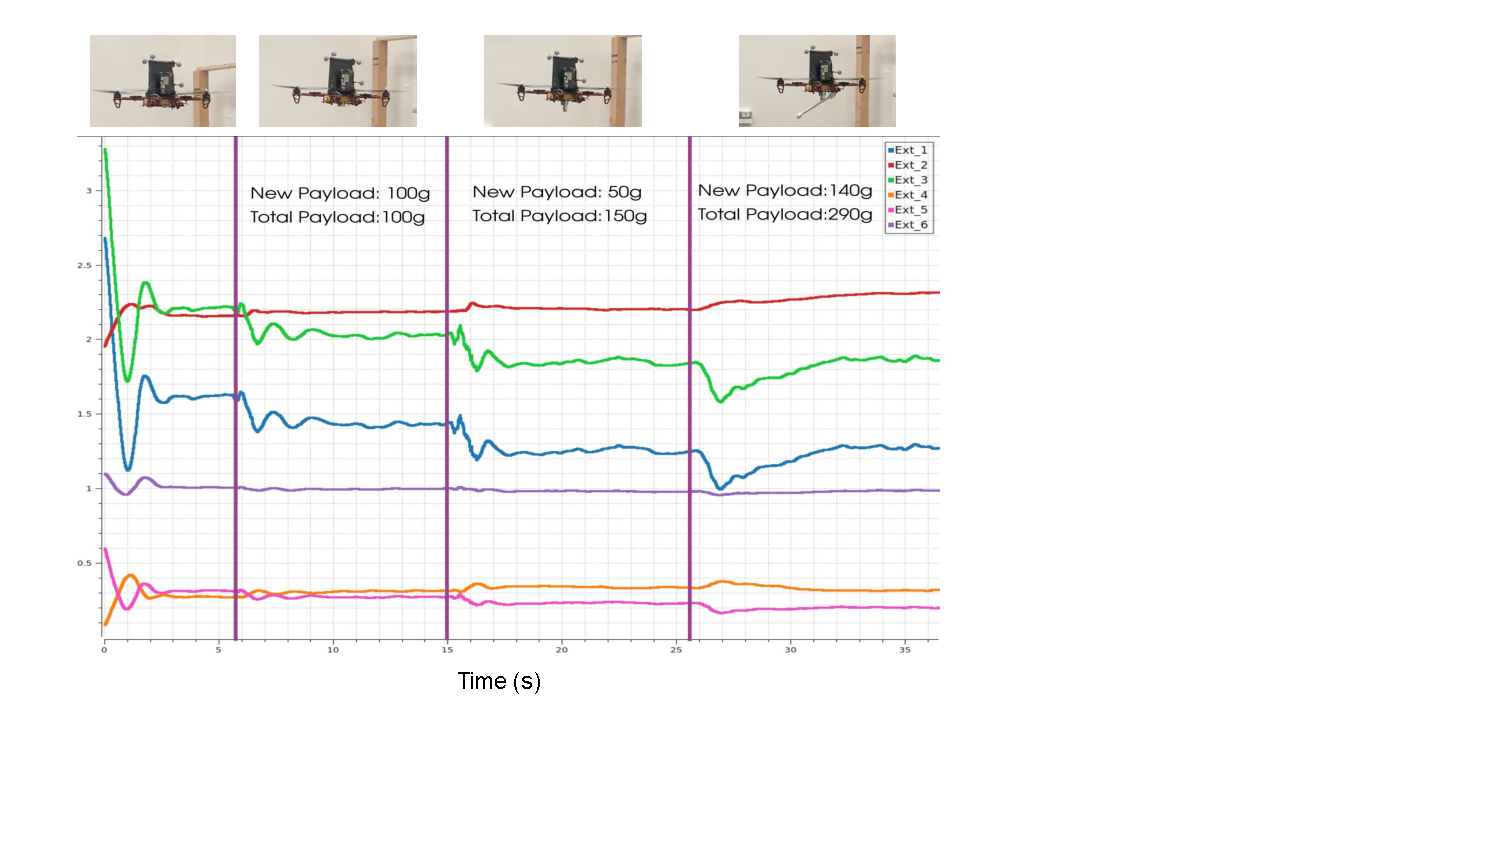
\includegraphics[width=\columnwidth]{img/extrinsics_plot_timescale.pdf}
    \caption{We analyze the change in behaviour of our policy as we incrementally add total 290g payloads to our quadcopter. We plot all 6 components of the intrinsics vector $\hat{z_t}$ predicted by the adaptation module. We see that changes in intrinsics are strongly correlated with disturbances applied to the quadcopter, indicating that the added payloads have been detected by the adaptation module. When the payload is added, the quadcopter first sinks and then recovers to the normal motion. The plotted components of the intrinsics vector change in response to the disturbance, from which we know the adaptation period takes around 2s.}
    \label{fig:intrinsics_analysis}
\end{figure}
%
Still, explicitly regressing the environment vector $e_t$, instead of its low-dimensional representation $z_t$, scarifies the success rate since it is trying to solve a harder estimation problem which is not necessary to solve the task at hand.
%
Since the tracking errors are computed only for successful runs, the \emph{SysID} baseline achieves a slightly lower tracking error in one of the metrics.
%
$\mathcal{L}1$ is the baseline with the strongest performance in our simulation experiments. However, it relies on the explicit knowledge of a reference model which we choose as the median value of all parameters in the testing range in Table~\ref{tab:randomization}, while our method with other baselines has no prior knowledge of the model. 
%
% The comparison between our method and $\mathcal{L}1$ shows that it is not enough to achieve adaptive control across platforms by estimating and compensating large model variance in model dynamics from a reference model. 
However, $\mathcal{L}1$ is not implemented in our real-world experiments as a baseline because it is highly sensitive to latency and requires significant engineering work. In contrast, our approach can handle latency very well by simulating it during training.
%
We also evaluate the task of stabilization on held-out environmental disturbances, as exemplified by random external forces and partial failure of a motor. The results of these experiments are reported in Table~\ref{tab:sim-metrics-unseen-disturb}. Our method outperforms all baselines in both out-of-distribution disturbances cases. Compared to the strongest baseline $\mathcal{L}1$, our method reduces the failure rate by up to 1.14 times, the average height error by up to 67.7\%,  and the average command tracking error by up to 22.4\%. 

% %
% Given the very large amount of quadcopter variations, the policy trained without access to environment parameters fails to achieve reasonable performance. This is because it is forced to learn a single conservative flying which can fly all quadcopters under varying disturbances.
% %
% Indeed, it either crashes to the ground or flies outside of the flying region.
% %
% Conversely, with access to environment parameters, the flight performance strongly increases.
% %
% Still, explicitly regressing the environment vector $e_t$, instead of its low-dimensional representation $z_t$ scarifies the success rate since it is trying to solve a harder estimation problem which is not necessary to solve the task at hand.
% %
% Since the tracking errors are computed only for successful runs, the \emph{SysID} baseline achieves a slightly lower tracking error on one of the metrics.
% %
% Having to solve additional scenarios which are potentially more challenging, our method accumulates a higher error, but still manages to keep the quadcopter from crashing.

% Our experiments show that whenever the policy  the importance of online adaptation.
% %
% We create a large 


\subsection{Adaptation Analysis}
We analyze the estimated intrinsics vector $\hat{z_t}$ for adaptation on incremental payloads. We incrementally add payloads in total of 290g to the quadcopter in hovering. The quadcopter adapts successfully to payloads and stabilizes itself at the target position. 
%
We plot all components of the estimated intrinsics vector from the adaptation module during the experiment in Figure~\ref{fig:intrinsics_analysis}. 
%
We find that whenever a payload is applied, there is a change in all intrinsics components, indicating that the disturbance has been detected by the adaptation module. 
%
Then the quadcopter recovers from the disturbance and all components of the intrinsics vector converges to different values as they are before the payload is applied. 
% It shows that even after adaptation, the adaptation module still detects the existence of payloads. 
%
From the change of the plotted components of intrinsics vector in response to the disturbance, we see that it takes around 2s for our controller to detect the disturbance, estimate the intrinsics vector, adapts from the disturbance, and finally stablizes. 
%
The adaptation period of our controller is much faster than that of methods with online estimation of ground truth model parameters such as~\cite{wuest2019online}, where it takes 10s to 15s in-flight to obtain an accurate model estimate.

\section{Conclusion}
In this work, we show how a single policy can control quadcopters of totally different size, mass, and actuation. 
%
We successfully transfer a method initially developed for legged locomotion in adapting terrains to quadcopters in adapting a diverse set of quadcopter bodies and disturbances.
%
Without any additional tuning or modification, the single policy trained only in simulation can be deployed zero-shot to quadcopters of very different design and hardware characteristics while showing rapid adaptation to unknown disturbances at the same time.
%
However, our current controller is a quasi-static position controller which fails on tracking aggressive flights. 
%
Future work should focus on improving its ability to track arbitrary trajectories to achieve a universal quadcopter controller. 
% Adaptive control has achieved great success in adaptation to model uncertainties and disturbances, but our work offers a fresh view on the meaning of adaptation by completely bypassing the notion of a \emph{reference} model that most adaptive control methods use. 
%
%while additionally showing rapid adaptation to unknown payloads during deployment. It differs from classic adaptative control in that it does not compensates for disparities between observations and the referenced model.
%
% This feature enables our method to adapt to a much wider range of robots and disturbances.
%
%
% One limitation of our approach is that it relies on simulation to improve, necessitating the need to replicate and train on situations in the simulation in which it might fail to work in the real world. A more scalable lifelong solution to the problem would be to continuously learn in the real world with the data collected during deployment in the real world. 
%
% \propose{Future work will aim to incorporate learning with real world data into the method. }
%
%In addition, we noticed a trade-off between the tracking performance and the probability of crashing. In this work, we favoured safety to tracking error. 
%and the  the policy presented in this paper is trained to take avoiding crashes at the time of adaptation as the priority out of other goals including tracking high-level commands. 
%However, future work will aim to relax this trade-off. 
%However, in the near future, we will have to improve the tracking performance and ensure safety.  

\section{Acknowledgement}
This work was supported by the DARPA Machine Common Sense program, Hong Kong Center for Logistics Robotics, and the Graduate Division Block Grant of the Dept. of Mechanical Engineering, UC Berkeley.
 The experimental testbed at the HiPeRLab is the result of contributions of many people, a full list of which can be found at \url{hiperlab.berkeley.edu/members/}. This work was also partially supported by the ONR MURI award N00014-21-1-2801.



%===============================================================================

% The maximum paper length is 8 pages excluding references and acknowledgements, and 10 pages including references and acknowledgements

%\clearpage
% The acknowledgments are automatically included only in the final and preprint versions of the paper.
% \acknowledgments{}

%===============================================================================

% no \bibliographystyle is required, since the corl style is automatically used.
% \bibliography{references.bib}  % .bib

\bibliographystyle{IEEEtran}
\bibliography{references}



\end{document}
